\chapter{DESAIN SISTEM}

\section{DESKRIPSI SOLUSI}

Solusi fundamental yang diajukan dalam proyek akhir ini adalah membangun sebuah platform digital terintegrasi bernama InternSync. Platform ini hadir sebagai solusi mutakhir untuk mengikis habis ketidakefektifan pengawasan manual dan lambatnya birokrasi logbook fisik yang selama ini terjadi di SMK PGRI Telagasari. Secara argumentatif, InternSync menawarkan keunggulan fungsionalitas melalui fitur-fitur taktis berikut:

\begin{itemize}
\item \textbf{Akses Web Responsif Terpusat:} Menyediakan akses web responsif (CMS) untuk seluruh aktor pengguna sekolah, sehingga Siswa dapat mengisi laporan harian di lokasi magang dan Guru Pembimbing dapat memantau siswa di lapangan melalui peramban ponsel. Aplikasi mobile berbasis Flutter direncanakan sebagai pengembangan lanjutan (subbab 3.3).
\item \textbf{Katalog Lowongan Industri Terpadu:} Data master industri mitra dan dokumen MoU ditambahkan oleh Hubin, sedangkan pembagian lowongan (meliputi kuota, jenis umum atau khusus jurusan, posisi, dan deskripsi lowongan) diatur oleh Koordinator PKL. Siswa dapat melihat katalog dan melamar lowongan yang sesuai dengan kompetensi keahliannya, kemudian Koordinator menyeleksi pendaftar tersebut sebelum penempatan diajukan secara resmi kepada Hubin.
\item \textbf{Pemantauan Presensi dan Perizinan Nir-Hambat:} Mengintegrasikan alur perizinan presensi (izin/sakit) yang memfasilitasi persetujuan pembimbing industri secara instan melalui tautan aman ber-token tanpa perlu login, didukung mekanisme fallback verifikasi guru pembimbing agar proses administrasi tidak menjadi penghambat.
\item \textbf{Monitoring Jurnal Harian (Logbook) Digital Mandiri:} Memfasilitasi pencatatan aktivitas kerja harian mandiri siswa (\textit{self-reporting}) secara terstruktur beserta unggahan bukti kegiatan yang terhubung dengan penguncian tanggal izin/sakit otomatis, dipantau secara berkala oleh Guru Pembimbing serta dilengkapi fitur ekspor rekapitulasi PDF ber-QR Code resmi untuk arsip sekolah.
\item \textbf{Evaluasi Terstandarisasi Berbasis Rubrik Baku:} Mempercepat kompilasi nilai evaluasi PKL yang mengadopsi rubrik baku jurnal PKL SMK (mencakup aspek non-teknis/sikap dan aspek teknis/keterampilan dari industri serta laporan sekolah) secara otomatis dan akurat.
\end{itemize}

\section{PERANCANGAN SISTEM}

\subsection{Rancangan Arsitektur Sistem}

Arsitektur sistem pada aplikasi manajemen Praktik Kerja Lapangan (PKL) InternSync dirancang menggunakan pendekatan arsitektur \textit{three-tier} (\textit{Client Tier}, \textit{Application Tier}, dan \textit{Data Tier}) berbasis RESTful API yang memisahkan secara tegas antara lapisan antarmuka pengguna (\textit{presentation layer}), lapisan logika bisnis (\textit{business logic layer}), dan lapisan penyimpanan data (\textit{persistence layer}). Pendekatan ini bertujuan untuk memisahkan tanggung jawab setiap komponen sistem sehingga pengelolaan data, pemrosesan aturan bisnis, serta penyajian antarmuka lintas platform dapat berjalan secara terstruktur dan mudah dikembangkan.

Pada lapisan \textit{Client Tier}, interaksi pengguna dibagi ke dalam dua kanal akses yang telah diimplementasikan. Pertama, Aplikasi Web CMS yang dibangun menggunakan React.js, TypeScript, dan Tailwind CSS untuk mengakomodasi lima aktor internal sekolah yang memiliki akun, yaitu Admin Sistem, Waka Hubin, Koordinator PKL, Guru Pembimbing, dan Siswa. Kedua, Antarmuka Web Publik berbasis rute token unik (\textit{public route}) yang memungkinkan Pembimbing Industri memberikan persetujuan izin/sakit serta menginput penilaian rubrik tanpa perlu melakukan login akun. Selain itu, Aplikasi Mobile berbasis Flutter (Dart) bagi Siswa dan Guru Pembimbing direncanakan sebagai kanal akses tambahan yang akan memakai REST API yang sama dan belum diimplementasikan pada proyek akhir ini.

\begin{figure}[H]
\centering
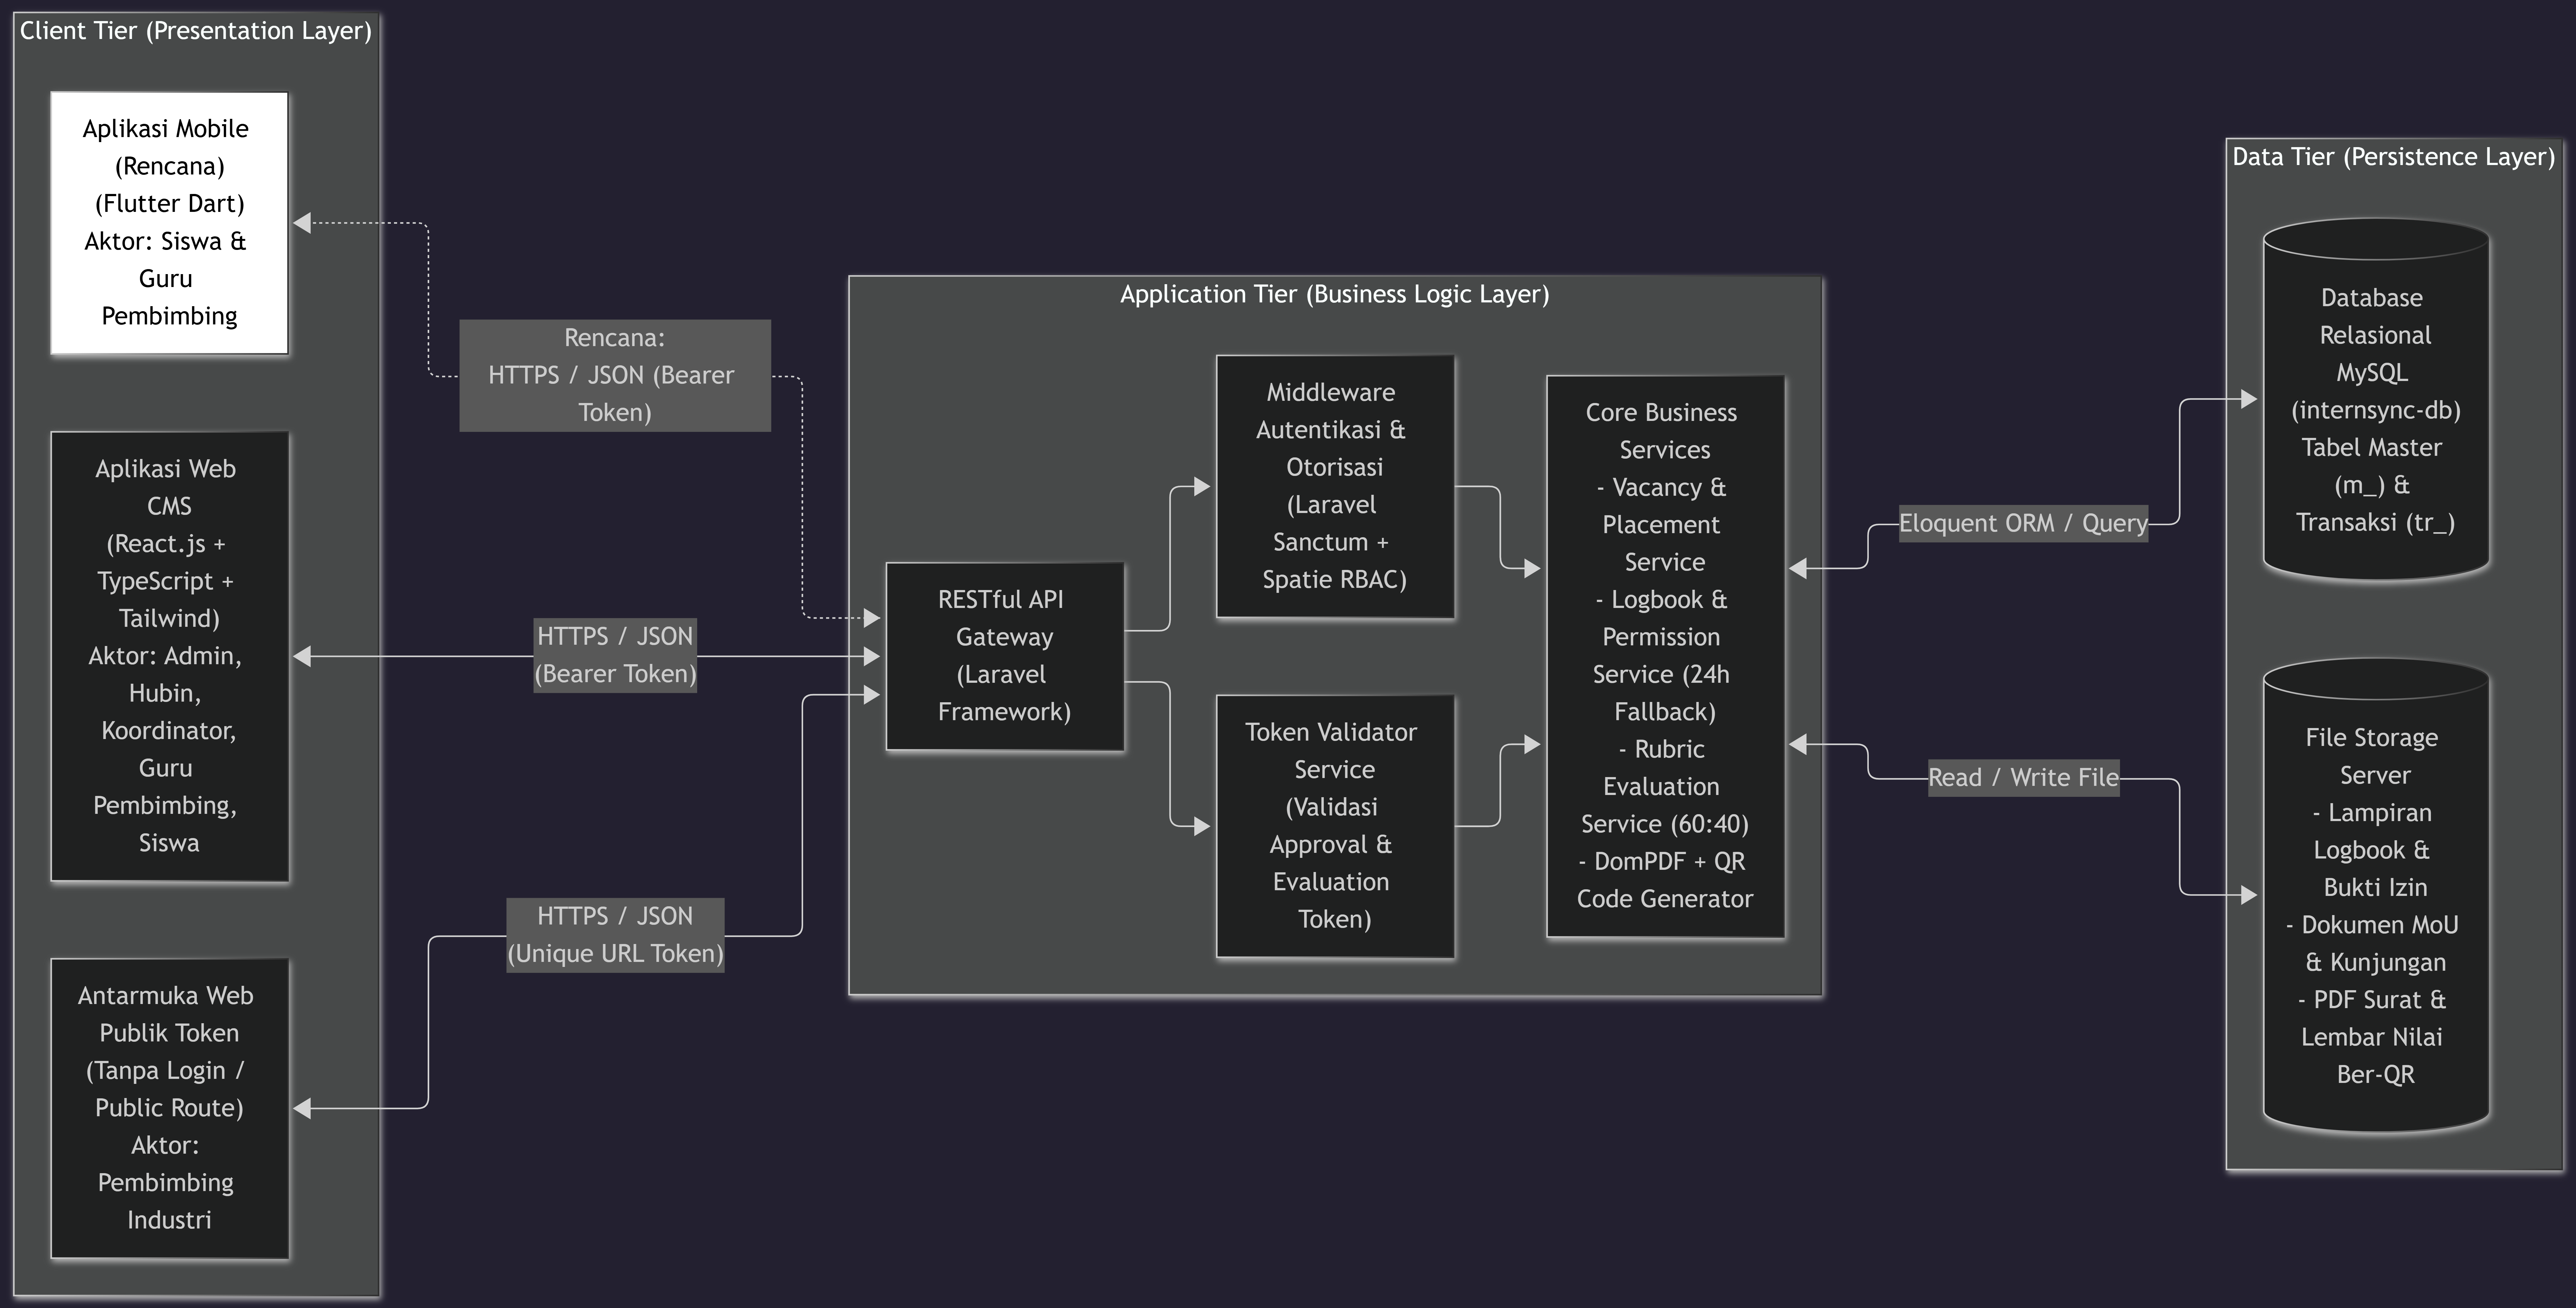
\includegraphics[width=12.39cm,height=0.78\textheight,keepaspectratio]{gambar/gambar-3-01.png}
\caption{Desain Arsitektur Sistem}\label{fig:3.1}
\end{figure}

Berdasarkan Gambar 3.1, proses komunikasi data dimulai ketika aplikasi web (dan kelak aplikasi mobile) mengirimkan permintaan melalui protokol HTTPS dalam format JSON yang diamankan dengan \textit{Bearer Token}, sedangkan antarmuka publik industri berkomunikasi menggunakan parameter \textit{Unique URL Token}. Seluruh permintaan diterima oleh \textit{RESTful API Gateway} berbasis framework Laravel pada \textit{Application Tier}. Permintaan dari aktor berakun akan melewati \textit{Middleware Autentikasi dan Otorisasi} (Laravel Sanctum dan Spatie RBAC), sementara akses publik industri akan divalidasi oleh \textit{Token Validator Service}. Selanjutnya, permintaan diproses oleh \textit{Core Business Services} yang mencakup layanan katalog lowongan dan penempatan, layanan \textit{self-reporting logbook} dan perizinan dengan aturan \textit{fallback} 24 jam, layanan evaluasi rubrik (rasio 60:40), serta generator dokumen DomPDF dan QR Code. Pada lapisan \textit{Data Tier}, sistem memanfaatkan Eloquent ORM untuk berkomunikasi dengan basis data relasional MySQL (\texttt{internsync-db}) yang memisahkan tabel master (\texttt{m\_}) dan tabel transaksi (\texttt{tr\_}), serta terhubung dengan \textit{File Storage Server} untuk menyimpan lampiran bukti logbook, surat izin, dokumen MoU, dan berkas PDF resmi ber-QR Code.

\subsection{Business Process Model and Notation (BPMN)}

BPMN digunakan untuk memberikan gambaran visual mengenai urutan aktivitas bisnis secara end-to-end yang melibatkan berbagai aktor di SMK PGRI Telagasari. Diagram ini memetakan kolaborasi antara Hubin, Koordinator, Pembimbing, dan Siswa dalam satu alur kerja terpadu.

\begin{figure}[H]
\centering
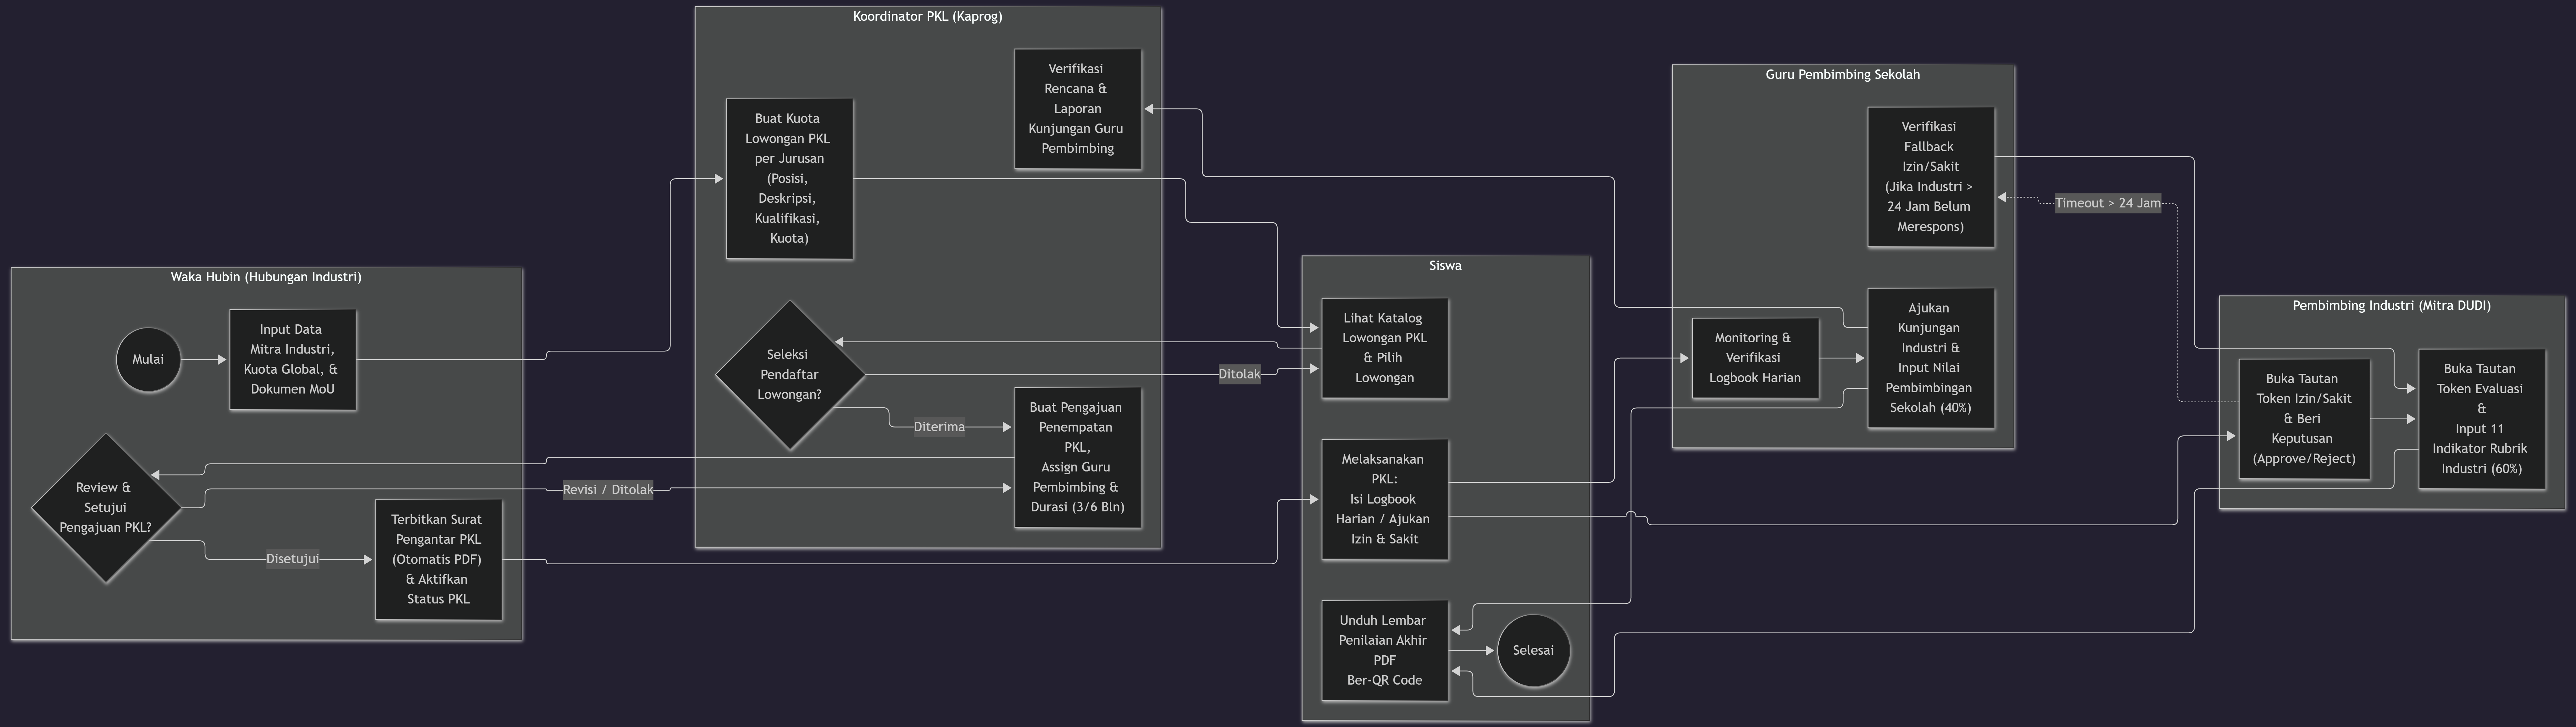
\includegraphics[width=13.98cm,height=0.78\textheight,keepaspectratio]{gambar/gambar-3-02.png}
\caption{Business Process Model and Notation (BPMN)}\label{fig:3.2}
\end{figure}

Berdasarkan Gambar~\ref{fig:3.2}, alur bisnis dimulai dari Waka Hubin yang menginput data master mitra industri serta dokumen MoU. Koordinator PKL kemudian mengatur lowongan PKL pada industri tersebut yang mencakup kuota, jenis lowongan (umum atau khusus jurusan), posisi, dan deskripsi. Siswa melihat katalog lowongan dan mengajukan lamaran pada lowongan yang diminati, lalu Koordinator menyeleksi siswa pendaftar lowongan tersebut. Apabila ditolak, siswa dapat memilih kembali lowongan lain yang tersedia; apabila diterima, Koordinator membuat dokumen pengajuan dan pengiriman PKL disertai penunjukan Guru Pembimbing dan penetapan durasi (3 atau 6 bulan) untuk ditinjau oleh Waka Hubin. Jika disetujui, Hubin menerbitkan Surat Pengantar PKL otomatis berformat PDF dan mengaktifkan status PKL siswa.

Selama masa pelaksanaan PKL, siswa mengisi \textit{logbook} harian secara mandiri atau mengajukan permohonan izin dan sakit. Catatan \textit{logbook} harian dipantau oleh Guru Pembimbing Sekolah dan dapat diekspor menjadi rekapitulasi PDF ber-QR Code, sedangkan permohonan izin/sakit diteruskan kepada Pembimbing Industri melalui tautan token untuk diberikan keputusan (\textit{approve/reject}). Apabila dalam waktu lebih dari 24 jam pihak industri belum merespons (\textit{timeout}), wewenang verifikasi izin dialihkan ke mekanisme \textit{fallback} oleh Guru Pembimbing Sekolah. Selain itu, Guru Pembimbing melaksanakan kunjungan industri berdasarkan jadwal Surat Perintah Perjalanan Dinas (SPPD) yang ditetapkan oleh Koordinator PKL. Pada tahap akhir, Pembimbing Industri menginput nilai pada 9 indikator rubrik industri (bobot 60\%) melalui tautan token evaluasi, dan Guru Pembimbing menginput nilai pada 2 indikator akademik sekolah (bobot 40\%), sehingga total terdapat 11 indikator penilaian. Setelah seluruh indikator terisi, sistem menghitung nilai akhir sehingga siswa dapat melihatnya serta mengunduh lembar penilaian berformat PDF.

\subsection{Use Case Diagram}

Use Case Diagram menggambarkan fungsionalitas sistem dari perspektif pengguna. Diagram ini mendefinisikan batasan sistem dan interaksi aktor terhadap fitur-fitur utama yang dikembangkan.

\begin{figure}[H]
\centering
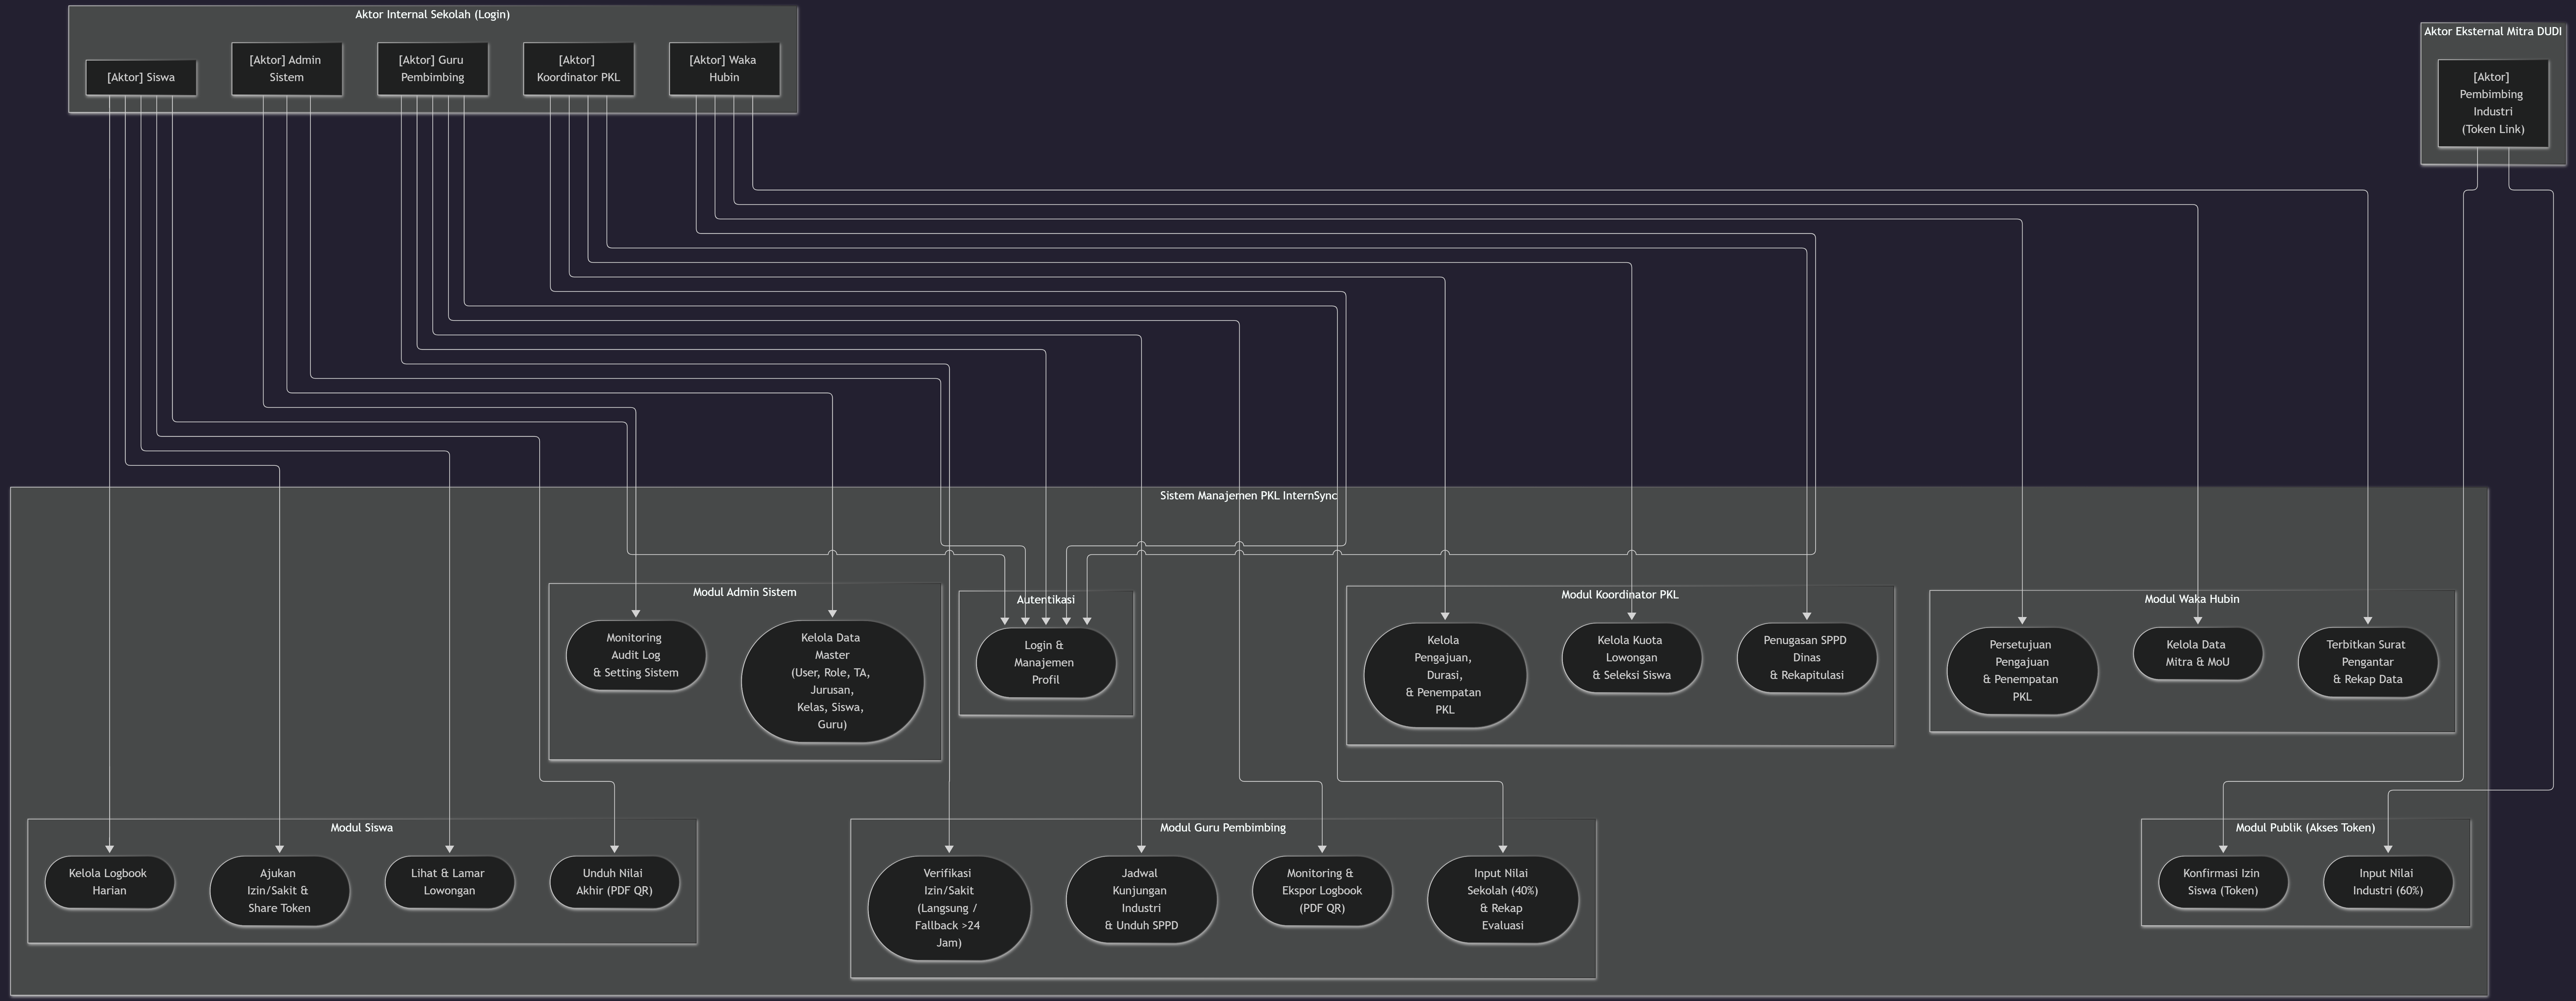
\includegraphics[width=13.98cm,height=0.78\textheight,keepaspectratio]{gambar/gambar-3-03.png}
\caption{Use Case Diagram}\label{fig:3.3}
\end{figure}

Terdapat lima aktor internal sekolah yang memiliki akun login dan satu aktor eksternal mitra DUDI tanpa login, dengan rincian fungsionalitas per modul sebagai berikut:

\begin{enumerate}[label=\alph*.]
\item \textbf{Admin Sistem:} Mengakses modul autentikasi (login dan manajemen profil), mengelola seluruh data master sistem (meliputi data \textit{user}, \textit{role}, tahun ajaran, jurusan, kelas, siswa, dan guru), serta melakukan \textit{monitoring audit log} dan pengaturan sistem.
\item \textbf{Waka Hubin (Hubungan Industri):} Mengakses modul autentikasi, mengelola data mitra industri dan dokumen MoU, melakukan persetujuan pengajuan dan penempatan PKL dari koordinator, serta menerbitkan surat pengantar PKL resmi dan memantau rekap data PKL.
\item \textbf{Koordinator PKL:} Mengakses modul autentikasi, mengelola kuota lowongan PKL dan menyeleksi siswa pendaftar, mengelola pengajuan, pengiriman, dan durasi PKL (3 atau 6 bulan), serta mengelola penugasan perjalanan dinas (SPPD) dan rekapitulasi laporan.
\item \textbf{Guru Pembimbing:} Mengakses modul autentikasi, melakukan \textit{monitoring} dan mengekspor \textit{logbook} harian siswa ke format PDF ber-QR Code, memverifikasi izin/sakit siswa (secara langsung maupun melalui mekanisme \textit{fallback} lebih dari 24 jam), melihat jadwal kunjungan industri dan mengunduh SPPD, serta menginput nilai sekolah (40\%) dan merekap evaluasi siswa.
\item \textbf{Siswa:} Mengakses modul autentikasi, melihat dan mengajukan lamaran pada katalog lowongan PKL, menginput dan mengelola \textit{logbook} harian secara mandiri, mengajukan permohonan izin/sakit beserta pembagian tautan token konfirmasi, serta melihat dan mengunduh lembar penilaian akhir berformat PDF ber-QR Code.
\item \textbf{Pembimbing Industri (Aktor Eksternal Mitra DUDI):} Berinteraksi tanpa login melalui modul publik berbasis tautan token untuk mengonfirmasi permohonan izin/sakit siswa serta menginput rubrik penilaian kinerja industri (bobot 60\%).
\end{enumerate}

\subsection{Activity Diagram}

Activity Diagram digunakan untuk menggambarkan alur aktivitas yang terjadi dalam sistem monitoring PKL berdasarkan interaksi antara pengguna dengan sistem. Diagram ini memodelkan proses yang dilakukan oleh setiap aktor melalui beberapa partisi atau swimlane yang menunjukkan pihak yang bertanggung jawab terhadap aktivitas tertentu. Dengan menggunakan Activity Diagram, alur proses sistem dapat dipahami secara lebih jelas mulai dari awal aktivitas hingga proses berakhir.

\subsubsection{Activity Diagram Login}

Activity Diagram login menggambarkan proses autentikasi pengguna sebelum dapat mengakses sistem monitoring PKL. Proses ini melibatkan interaksi antara pengguna yang memasukkan kredensial dan sistem yang melakukan validasi data.

\begin{figure}[H]
\centering
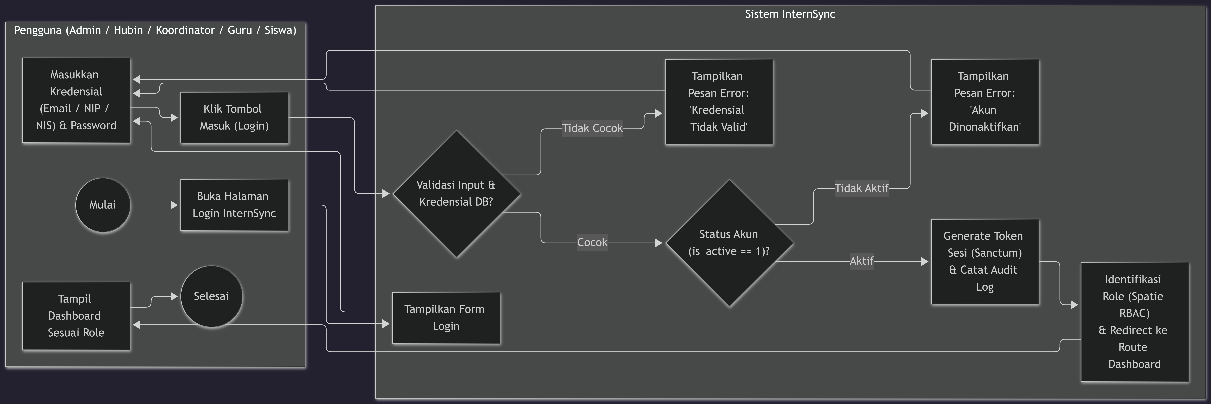
\includegraphics[width=13.98cm,height=0.78\textheight,keepaspectratio]{gambar/gambar-3-04.png}
\caption{Activity Diagram Login}\label{fig:3.4}
\end{figure}

Berdasarkan Gambar 3.4, proses dimulai ketika pengguna membuka halaman login InternSync, lalu sistem menampilkan formulir login. Pengguna memasukkan kredensial berupa Email, NIP, atau NIS beserta kata sandi dan menekan tombol masuk. Sistem melakukan validasi kecocokan kredensial terhadap basis data; apabila tidak cocok, sistem menampilkan pesan kesalahan \textit{Kredensial Tidak Valid} dan mengembalikan pengguna ke formulir login. Apabila kredensial cocok, sistem memeriksa status keaktifan akun (\texttt{is\_active == 1}). Jika akun berstatus tidak aktif, sistem menolak akses dan menampilkan pesan \textit{Akun Dinonaktifkan}. Jika akun aktif, sistem membuat token sesi autentikasi melalui Laravel Sanctum, mencatat aktivitas ke dalam tabel \textit{audit log}, mengidentifikasi peran pengguna melalui Spatie RBAC, dan mengarahkan pengguna ke halaman dasbor sesuai perannya masing-masing.

\subsubsection{Activity Diagram Katalog Lowongan dan Penempatan PKL}

Activity Diagram ini memvisualisasikan alur pengelolaan lowongan hingga penempatan siswa ke industri mitra. Proses ini penting untuk memastikan setiap siswa terdata secara sistematis di tempat pelaksanaan magang yang sesuai dengan keahliannya.

\begin{figure}[H]
\centering
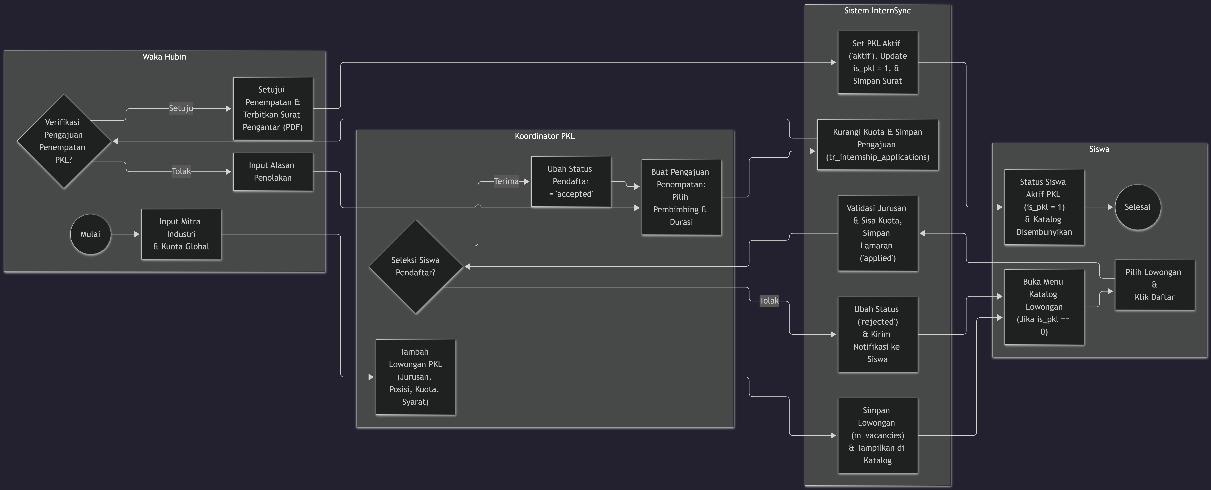
\includegraphics[width=13.98cm,height=0.78\textheight,keepaspectratio]{gambar/gambar-3-05.png}
\caption{Activity Diagram Katalog Lowongan dan Penempatan PKL}\label{fig:3.5}
\end{figure}

Proses diawali ketika Hubin menambahkan data industri mitra. Koordinator kemudian mengatur lowongan pada industri tersebut, meliputi kuota, jenis lowongan (umum atau khusus), posisi, dan deskripsi lowongan. Siswa dapat melihat katalog lowongan dan memilih lowongan yang diminati. Selanjutnya Koordinator menyeleksi siswa yang memilih lowongan, menetapkan penempatan beserta durasi pelaksanaan (3 atau 6 bulan), dan menunjuk guru pembimbing. Sistem memvalidasi input tersebut dan menyimpan dokumen pengajuan. Apabila validasi berhasil, pengajuan diteruskan kepada Hubin untuk disetujui, sehingga status magang siswa tercatat secara resmi untuk periode tersebut.

\subsubsection{Activity Diagram Pengisian Logbook}

Activity Diagram pengisian logbook menguraikan tahapan pencatatan aktivitas harian yang wajib dilakukan oleh siswa selama masa PKL. Logbook digital ini berfungsi sebagai portofolio capaian kompetensi harian yang dipantau secara berkala oleh guru pembimbing.

\begin{figure}[H]
\centering
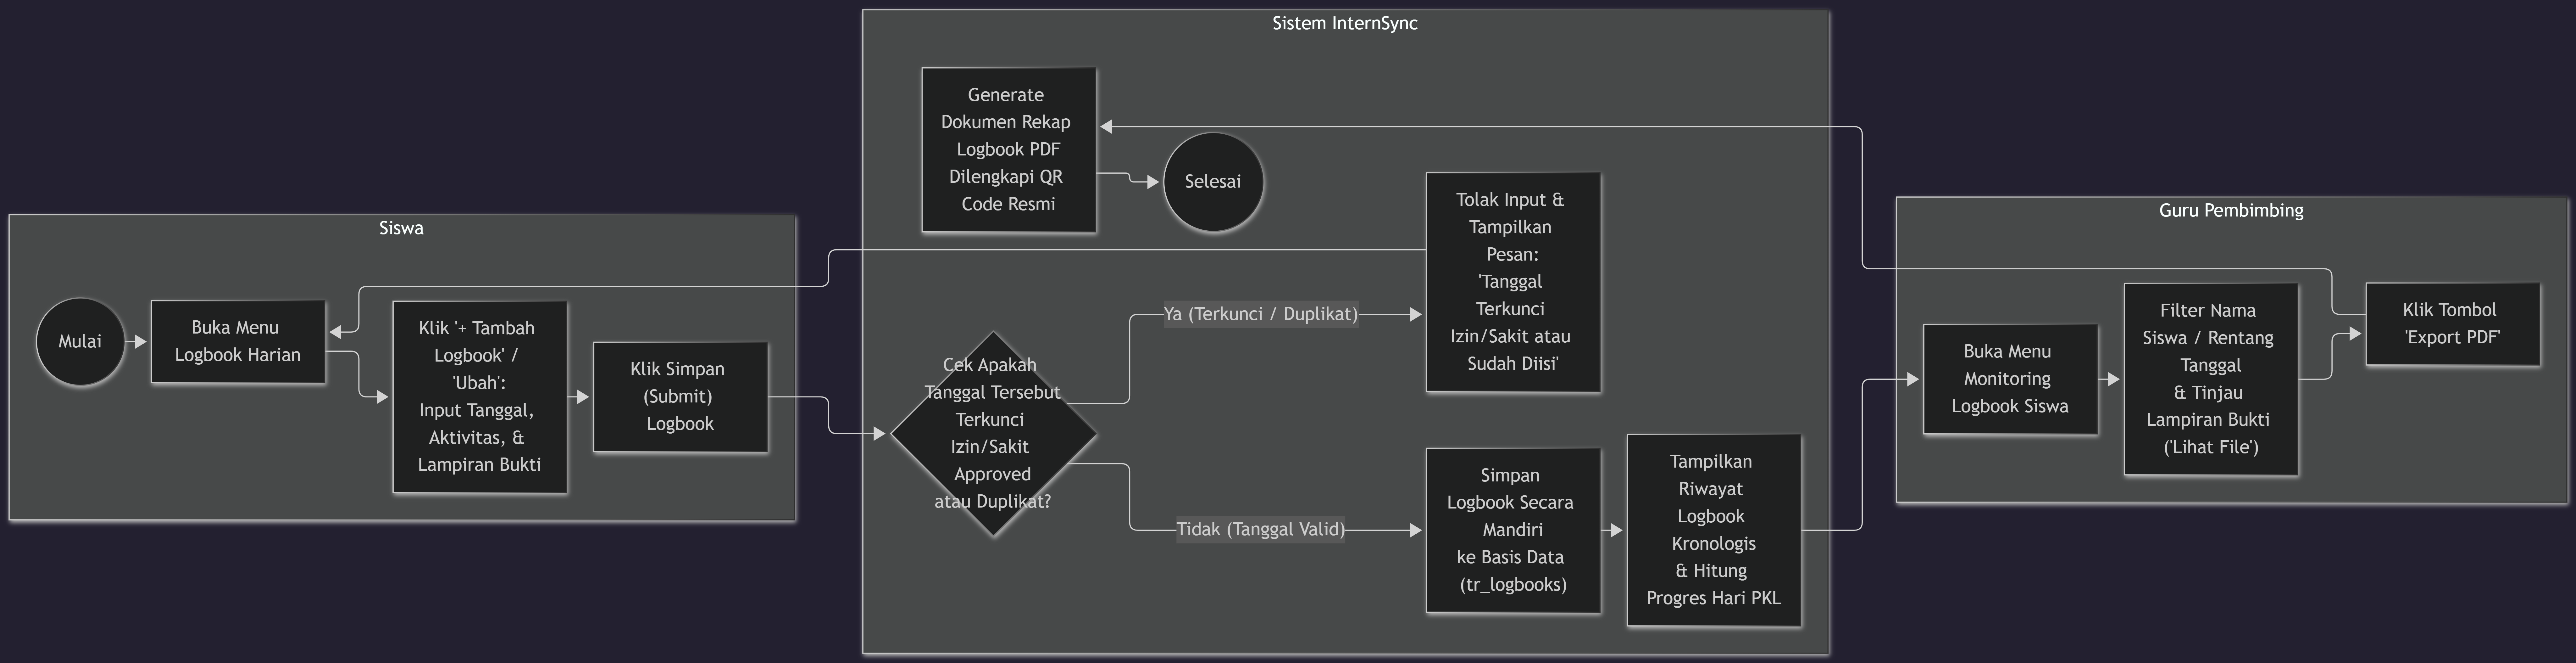
\includegraphics[width=13.98cm,height=0.78\textheight,keepaspectratio]{gambar/gambar-3-06.png}
\caption{Activity Diagram Pengisian Logbook}\label{fig:3.6}
\end{figure}

Berdasarkan Gambar 3.6, alur dimulai ketika siswa membuka menu \textit{logbook} harian dan menekan tombol tambah atau ubah \textit{logbook} untuk menginput tanggal, rincian aktivitas kerja, serta mengunggah berkas bukti pendukung. Setelah siswa menekan tombol simpan (\textit{submit}), sistem memeriksa apakah tanggal yang dipilih terkunci oleh status permohonan izin/sakit yang telah disetujui (\textit{approved}) atau telah terisi sebelumnya (duplikat). Apabila tanggal terkunci atau duplikat, sistem menolak input dan menampilkan pesan peringatan. Apabila tanggal valid, sistem langsung menyimpan catatan \textit{logbook} secara mandiri ke dalam tabel \texttt{tr\_logbooks}, menampilkan riwayat \textit{logbook} secara kronologis, serta memperbarui kalkulasi progres hari pelaksanaan PKL siswa. Selanjutnya, Guru Pembimbing dapat memantau seluruh entri aktivitas melalui menu \textit{monitoring logbook}, memfilter berdasarkan nama siswa atau rentang tanggal, meninjau lampiran bukti kegiatan, dan menekan tombol ekspor PDF untuk menghasilkan dokumen rekapitulasi \textit{logbook} resmi ber-QR Code.

\subsubsection{Activity Diagram Pengajuan Izin dan Sakit}

Activity Diagram pengajuan izin dan sakit mengatur mekanisme pelaporan ketidakhadiran siswa agar akuntabilitas kehadiran tetap terjaga tanpa menghambat operasional industri.

\begin{figure}[H]
\centering
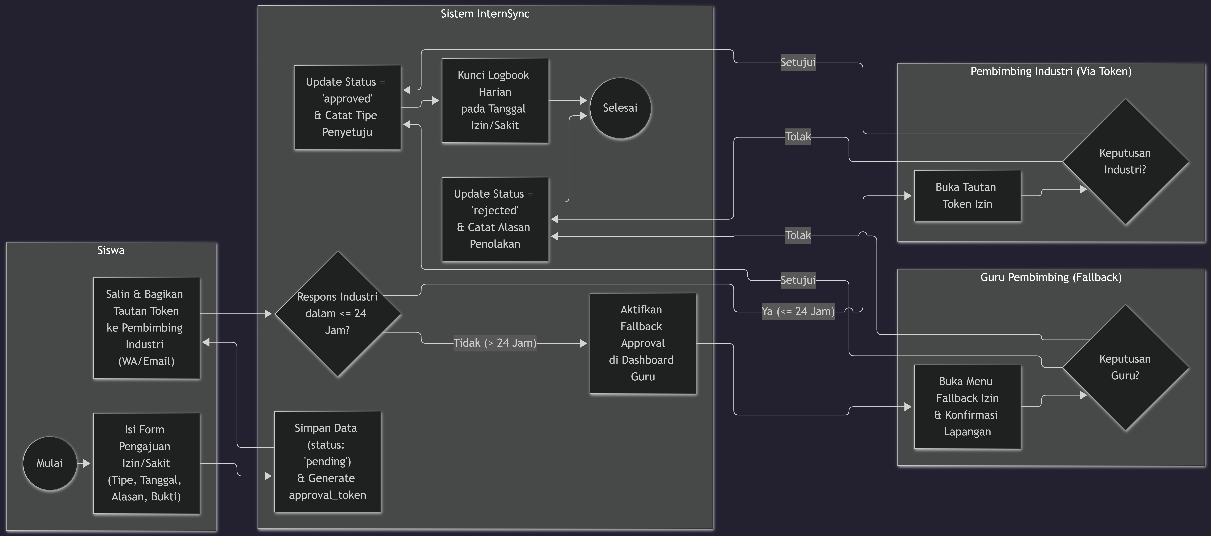
\includegraphics[width=13.99cm,height=0.78\textheight,keepaspectratio]{gambar/gambar-3-07.png}
\caption{Activity Diagram Pengajuan Izin dan Sakit}\label{fig:3.7}
\end{figure}

Alur dimulai saat siswa berhalangan hadir dan mengisi form perizinan pada sistem dengan memilih jenis ketidakhadiran (izin atau sakit), rentang tanggal, alasan, serta mengunggah dokumen bukti otentik (surat keterangan dokter atau surat izin orang tua). Sistem memvalidasi data dan secara otomatis mengirimkan notifikasi tautan ber-token aman kepada pembimbing industri. Pembimbing industri dapat langsung membuka tautan tersebut pada peramban ponsel dan memberikan persetujuan (approve/reject) dalam satu klik tanpa perlu melakukan login akun. Apabila dalam kurun waktu 24 jam pembimbing industri belum memberikan tanggapan, guru pembimbing sekolah memiliki hak akses fallback untuk memverifikasi izin tersebut secara langsung berdasarkan keabsahan dokumen bukti. Perizinan yang telah disetujui akan secara otomatis mengunci formulir logbook pada tanggal terkait sehingga siswa tidak tercatat alpa.

\subsubsection{Activity Diagram Evaluasi PKL}

Activity Diagram evaluasi PKL menggambarkan mekanisme penilaian akhir berbasis rubrik baku yang menjadi tolak ukur pencapaian kompetensi dan keberhasilan praktik kerja lapangan.

\begin{figure}[H]
\centering
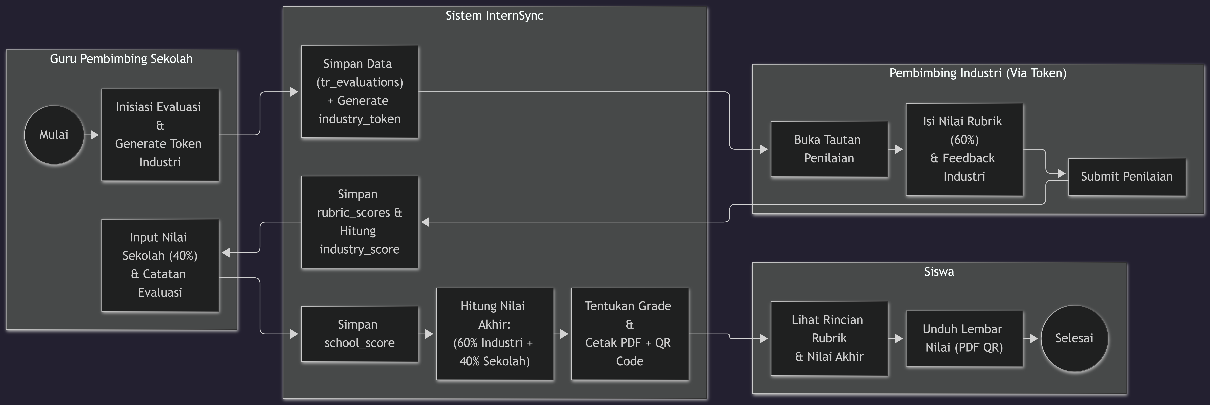
\includegraphics[width=13.97cm,height=0.78\textheight,keepaspectratio]{gambar/gambar-3-08.png}
\caption{Activity Diagram Evaluasi PKL}\label{fig:3.8}
\end{figure}

Evaluasi PKL mengadopsi standar rubrik baku jurnal PKL SMK dengan total 11 indikator dalam tiga kelompok. Kelompok A, aspek sikap dan non-teknis (5 indikator, dinilai industri), meliputi kedisiplinan dan kehadiran, tanggung jawab dan kejujuran, inisiatif dan kemandirian, etika kerja dan komunikasi tim, serta penerapan prosedur K3LH. Kelompok B, aspek keterampilan dan teknis (4 indikator, dinilai industri), meliputi penguasaan peralatan dan tooling industri, kualitas dan presisi hasil pekerjaan, kemampuan analisis dan pemecahan masalah, serta kecepatan dan ketuntasan tugas kerja. Kelompok C, aspek akademik dan laporan (2 indikator, dinilai sekolah), meliputi sistematika dan kelengkapan laporan akhir PKL serta penguasaan materi dan presentasi pertanggungjawaban. Pembimbing industri mengisi 9 indikator kelompok A dan B melalui tautan evaluasi aman, atau melalui lembar fisik yang kemudian diinputkan ke sistem oleh guru pembimbing saat kunjungan supervisi akhir, sedangkan guru pembimbing sekolah mengisi 2 indikator kelompok C. Sistem secara otomatis menghitung nilai industri dari 9 indikator dan nilai sekolah dari 2 indikator, menggabungkannya dengan bobot 60\% dan 40\% menjadi nilai akhir, mengonversinya ke predikat huruf (A, B, C, D), dan menerbitkan lembar penilaian akhir resmi yang dapat diakses dan diunduh siswa melalui dasbor masing-masing.

\subsection{Entity Relationship Diagram (ERD)}

Entity Relationship Diagram (ERD) merelasikan struktur basis data yang membentuk sistem monitoring PKL. Diagram ini memetakan entitas pengguna, siswa, industri, hingga pelaporan untuk memastikan komponen data saling terhubung dan terintegrasi dalam mendukung proses bisnis.

\begin{figure}[H]
\centering
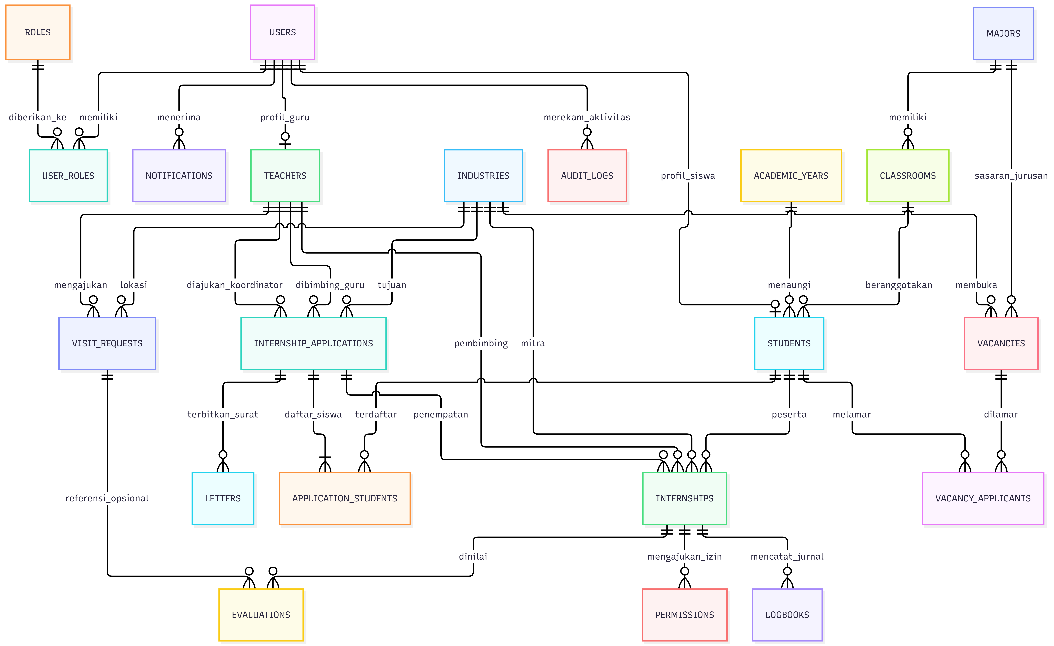
\includegraphics[width=12.17cm,height=0.78\textheight,keepaspectratio]{gambar/gambar-3-09.png}
\caption{Entity Relationship Diagram (ERD)}\label{fig:3.9}
\end{figure}

Berdasarkan Gambar 3.9, struktur entitas sistem menggunakan \texttt{USERS}, \texttt{ROLES}, dan \texttt{USER\_ROLES} untuk mengelola autentikasi dan hak akses multi-peran. Profil pengguna akademik dipetakan ke dalam entitas \texttt{STUDENTS} dan \texttt{TEACHERS}, yang didukung oleh entitas struktur akademik meliputi \texttt{ACADEMIC\_YEARS}, \texttt{MAJORS}, dan \texttt{CLASSROOMS}. Data kemitraan perusahaan disimpan pada entitas \texttt{INDUSTRIES}, yang berelasi dengan entitas \texttt{VACANCIES} dan \texttt{VACANCY\_APPLICANTS} untuk memfasilitasi katalog lowongan PKL serta seleksi pendaftar oleh koordinator. Proses pengajuan penempatan kelompok siswa dikelola melalui entitas \texttt{INTERNSHIP\_APPLICATIONS} dan \texttt{APPLICATION\_STUDENTS}, yang kemudian menghasilkan penempatan aktif pada entitas pusat \texttt{INTERNSHIPS} serta penerbitan dokumen surat resmi pada \texttt{LETTERS}. Selama pelaksanaan PKL, pencatatan kegiatan harian disimpan pada \texttt{LOGBOOKS}, pengajuan izin/sakit ber-token pada \texttt{PERMISSIONS}, penugasan supervisi lapangan guru pada \texttt{VISIT\_REQUESTS}, dan penilaian akhir berbasis rubrik pada \texttt{EVALUATIONS}. Sebagai pendukung tata kelola sistem, entitas \texttt{NOTIFICATIONS} menangani pesan pemberitahuan pengguna dan \texttt{AUDIT\_LOGS} merekam jejak aktivitas krusial demi menjaga akuntabilitas data.

Perancangan ERD yang baik berperan penting dalam memastikan relasi antar entitas berjalan secara konsisten serta meminimalkan redundansi data pada sistem \cite{ref14}. Penerapan Physical Data Model yang dinormalisasi turut mendukung efisiensi proses query serta menjaga integritas referensial antar tabel dalam basis data relasional \cite{ref15}.

\subsection{Physical Data Model (PDM)}

Physical Data Model (PDM) merupakan wujud implementasi struktur basis data secara nyata pada DBMS. Pemodelan ini mendeskripsikan secara detail tabel, atribut, tipe data, serta primary key yang akan mendukung keseluruhan proses pelaporan dan administrasi dalam sistem.

\begin{figure}[H]
\centering
\includegraphics[width=13.99cm,height=0.78\textheight,keepaspectratio]{gambar/gambar-3-10.png}
\caption{Physical Data Model (PDM)}\label{fig:3.10}
\end{figure}

{\raggedright
Perancangan fisik basis data pada Gambar 3.10 memisahkan secara tegas antara sepuluh tabel master (berawalan \texttt{m\_}) dan sebelas tabel transaksi (berawalan \texttt{tr\_}). Tabel master menyimpan referensi data yang relatif statis, mencakup \texttt{m\_users}, \texttt{m\_roles}, \texttt{m\_user\_roles}, \texttt{m\_academic\_years}, \texttt{m\_majors}, \texttt{m\_classrooms}, \texttt{m\_students}, \texttt{m\_teachers}, \texttt{m\_industries}, serta \texttt{m\_vacancies} (menyimpan katalog lowongan beserta kuota dan relasi opsional \texttt{major\_id} untuk lowongan umum maupun khusus jurusan). Sebaliknya, tabel transaksi mengakomodasi aktivitas operasional yang dinamis, meliputi \texttt{tr\_vacancy\_applicants}, \texttt{tr\_internship\_applications}, \texttt{tr\_application\_students}, \texttt{tr\_internships}, \texttt{tr\_logbooks}, \texttt{tr\_permissions} (dilengkapi atribut \texttt{approval\_token} dan \texttt{approved\_by\_type} untuk mekanisme \textit{fallback}), \texttt{tr\_visit\_requests}, \texttt{tr\_evaluations} (menyimpan matriks 11 indikator pada kolom JSON \texttt{rubric\_scores} dengan bobot \texttt{industry\_score} 60\% dan \texttt{school\_score} 40\%), \texttt{tr\_letters}, \texttt{tr\_notifications}, serta \texttt{tr\_audit\_logs}. Seluruh relasi operasional pelaksanaan magang berpusat pada tabel \texttt{tr\_internships} yang telah dinormalisasi hingga \textit{Third Normal Form} (3NF) guna menjaga integritas referensial dan menghindari redundansi data.
\par}

\subsection{Gambaran Antarmuka Sistem}

Gambar pada subbab ini merupakan tangkapan layar antarmuka sistem InternSync yang telah diimplementasikan. Gambar dipertahankan sesuai urutan siklus pelaksanaan Praktik Kerja Lapangan (PKL), mulai dari autentikasi dan pengelolaan data, seleksi serta penempatan siswa, hingga monitoring, evaluasi, dan pelaporan. Rangkaian gambar memperlihatkan tampilan antarmuka sekaligus alur penggunaan sistem oleh Admin, Hubin, Koordinator PKL, Guru Pembimbing, Siswa, dan Pembimbing Industri.

\subsubsection{Fase Autentikasi dan Administrasi Master Sistem}

Fase ini merupakan fondasi operasional sistem yang mencakup gerbang akses terpusat bagi seluruh pengguna serta tata kelola data master entitas yang dibutuhkan sebelum aktivitas PKL dapat diselenggarakan.

\begin{figure}[H]
\centering
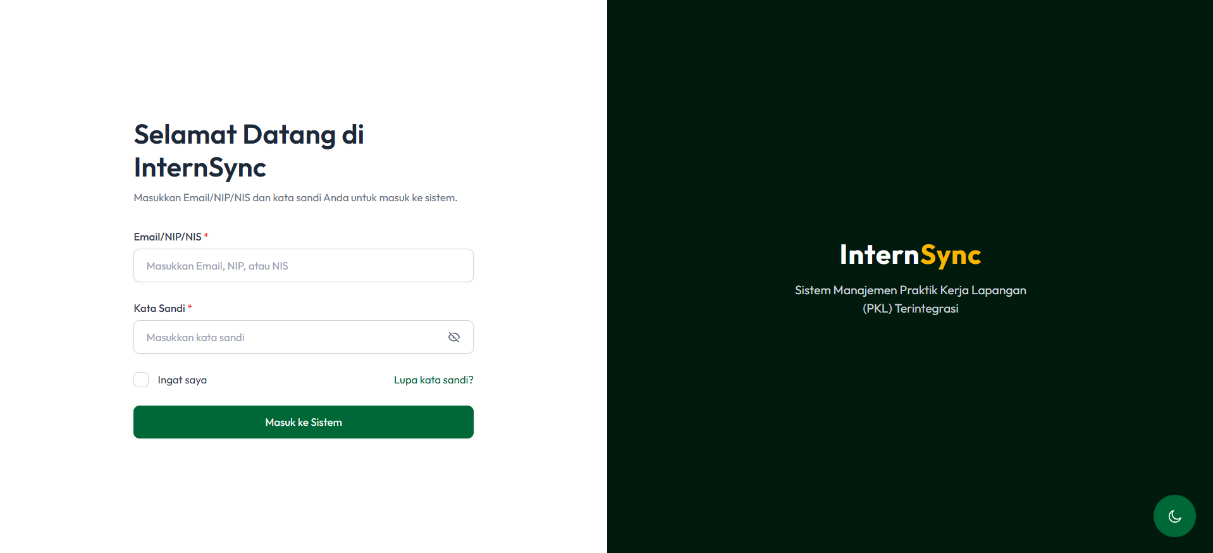
\includegraphics[width=14.00cm,height=0.78\textheight,keepaspectratio]{gambar/gambar-3-11.png}
\caption{Halaman Otentikasi (Login)}\label{fig:3.11}
\end{figure}

Antarmuka ini berfungsi sebagai pintu gerbang utama untuk mengakses sistem InternSync. Pengguna masuk dengan kredensial multiatribut berupa alamat email, NIP bagi tenaga pendidik, atau NIS bagi siswa, beserta kata sandi. Pada tampilan ini, formulir masuk di sisi kiri menyediakan fitur “Ingat Saya” dan opsi pemulihan kata sandi, sedangkan sisi kanan memuat logo InternSync, ilustrasi, dan ringkasan sistem. Sistem menggunakan Laravel Sanctum dan Spatie Role-Based Access Control (RBAC) untuk mengidentifikasi peran pengguna dan mengarahkan navigasi ke dasbor yang sesuai.

\begin{figure}[H]
\centering
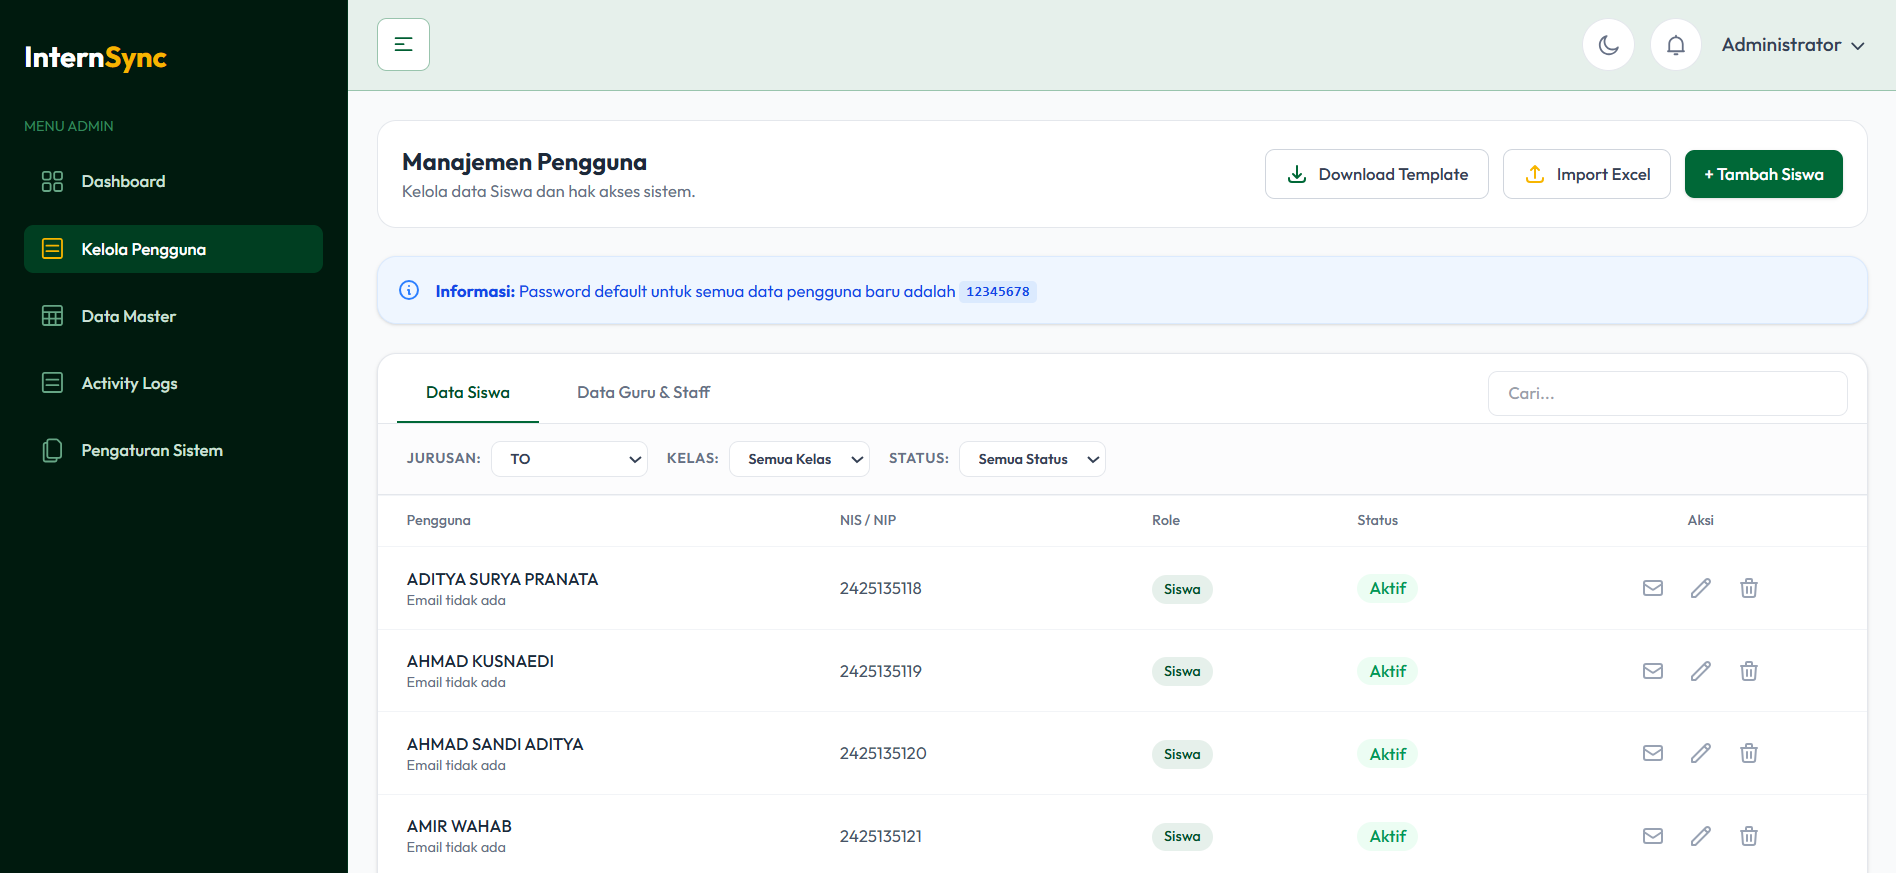
\includegraphics[width=14.00cm,height=0.78\textheight,keepaspectratio]{gambar/gambar-3-12.png}
\caption{Antarmuka Panel Administrasi dan Manajemen Pengguna (Admin)}\label{fig:3.12}
\end{figure}

Antarmuka ini merupakan pusat kendali manajemen akun yang diperuntukkan khusus bagi peran Admin Sistem pada menu Kelola Pengguna. Halaman ini memisahkan pengelolaan akun ke dalam dua tab terstruktur, yaitu tab Data Siswa dan tab Data Guru \& Staff, serta menampilkan informasi \textit{password default} bagi akun pengguna baru. Komponen utama antarmuka berupa \textit{data table} yang menyajikan daftar pengguna beserta atribut NIS/NIP, \textit{Role} (\textit{badge} Siswa/Guru), Status keaktifan akun (Aktif), serta kolom Aksi yang memuat tombol pintasan pengaturan email, ubah data (\textit{edit}), dan hapus akun. Untuk mempercepat migrasi data massal pada awal tahun ajaran, antarmuka ini dilengkapi fitur penyaringan berlapis (berdasarkan Jurusan, Kelas, dan Status), kolom pencarian cepat, serta tombol operasional \textit{Download Template}, \textit{Import Excel}, dan + Tambah Siswa di bagian kanan atas.

\begin{figure}[H]
\centering
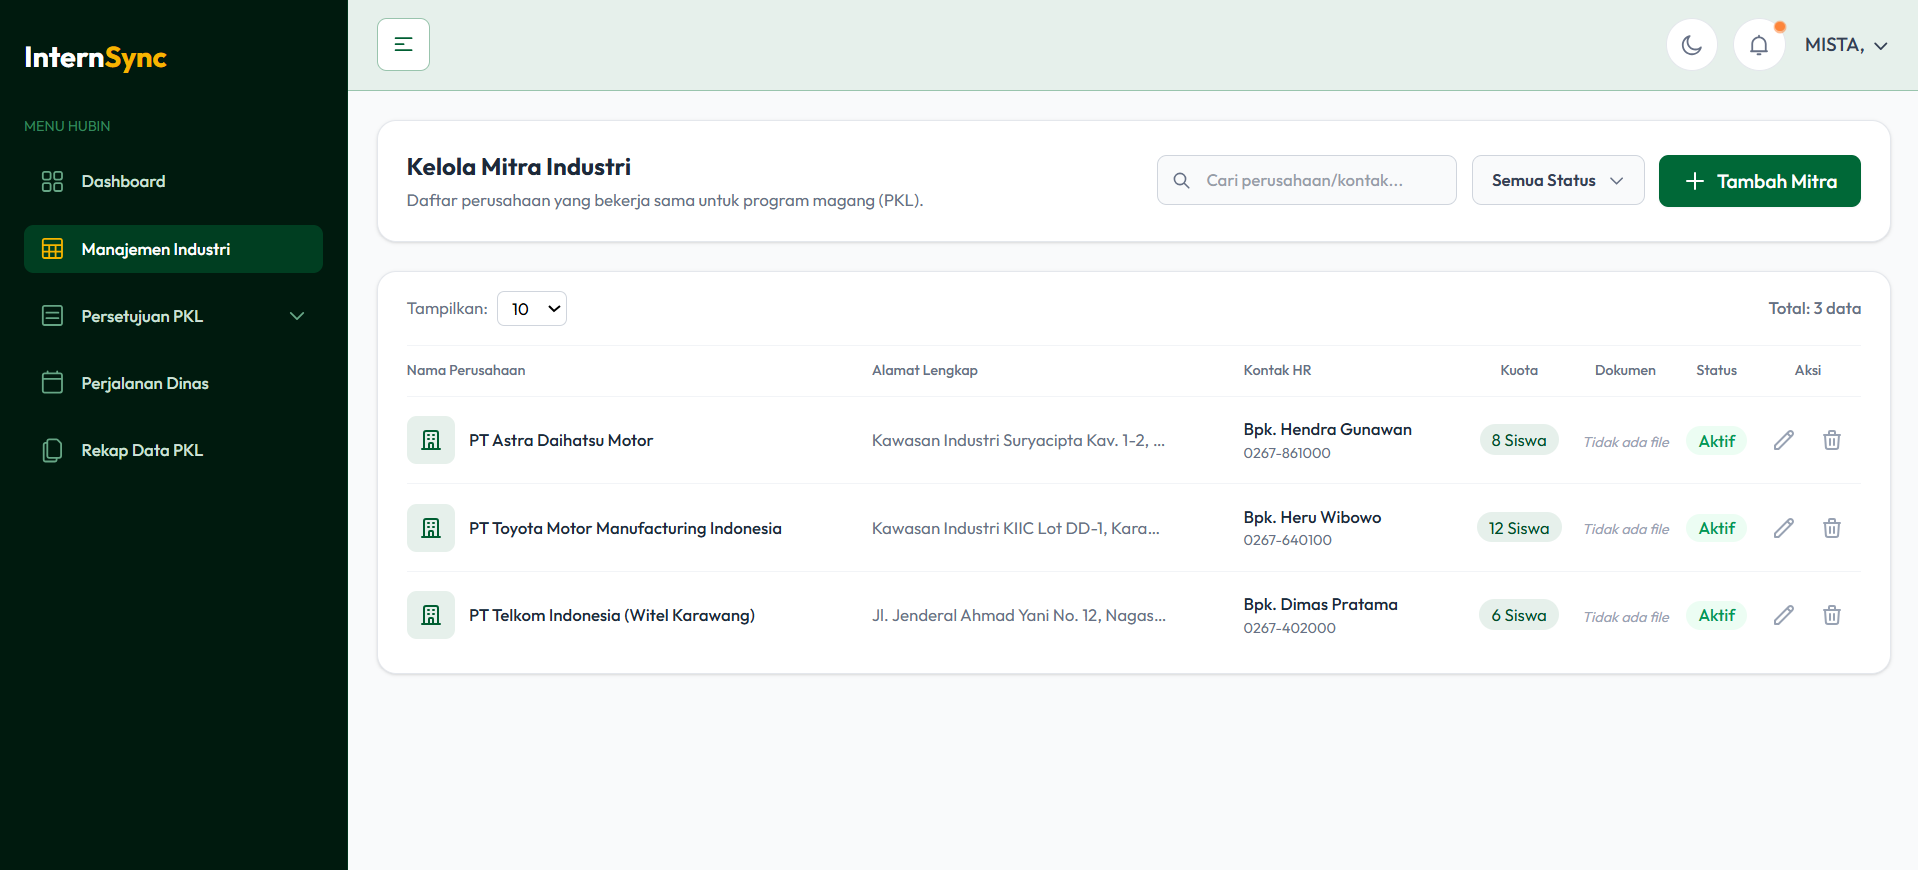
\includegraphics[width=14.00cm,height=0.78\textheight,keepaspectratio]{gambar/gambar-3-13.png}
\caption{Antarmuka Manajemen Mitra Industri dan Dokumen MoU (Hubin)}\label{fig:3.13}
\end{figure}

Antarmuka ini berfungsi sebagai modul tata kelola data master entitas dunia usaha dan dunia industri (DUDI) mitra yang berada di bawah wewenang Waka Hubin. Komponen utama menggunakan data table komprehensif yang memuat nama perusahaan, alamat operasional, kontak personal penanggung jawab/HR, status kerja sama aktif, serta kuota penempatan kumulatif. Dilengkapi dengan tombol aksi Tambah Mitra Baru, fasilitas unggah dokumen nota kesepahaman (MoU) legal dalam format digital, serta fitur modifikasi data secara inline. Ketersediaan data industri yang tervalidasi pada halaman ini menjadi prasyarat mutlak (prerequisite) bagi Koordinator PKL untuk dapat menginisiasi pembukaan lowongan PKL di tahap berikutnya.

\subsubsection{Fase Pra-PKL (Katalog Lowongan, Seleksi, Pengajuan, dan Penempatan)}

Fase ini mencakup rangkaian proses persiapan penempatan siswa, dimulai dari pembukaan kuota lowongan, pendaftaran mandiri oleh siswa, seleksi administratif, perumusan surat pengantar, hingga clearance keberangkatan resmi ke lokasi industri.

\begin{figure}[H]
\centering
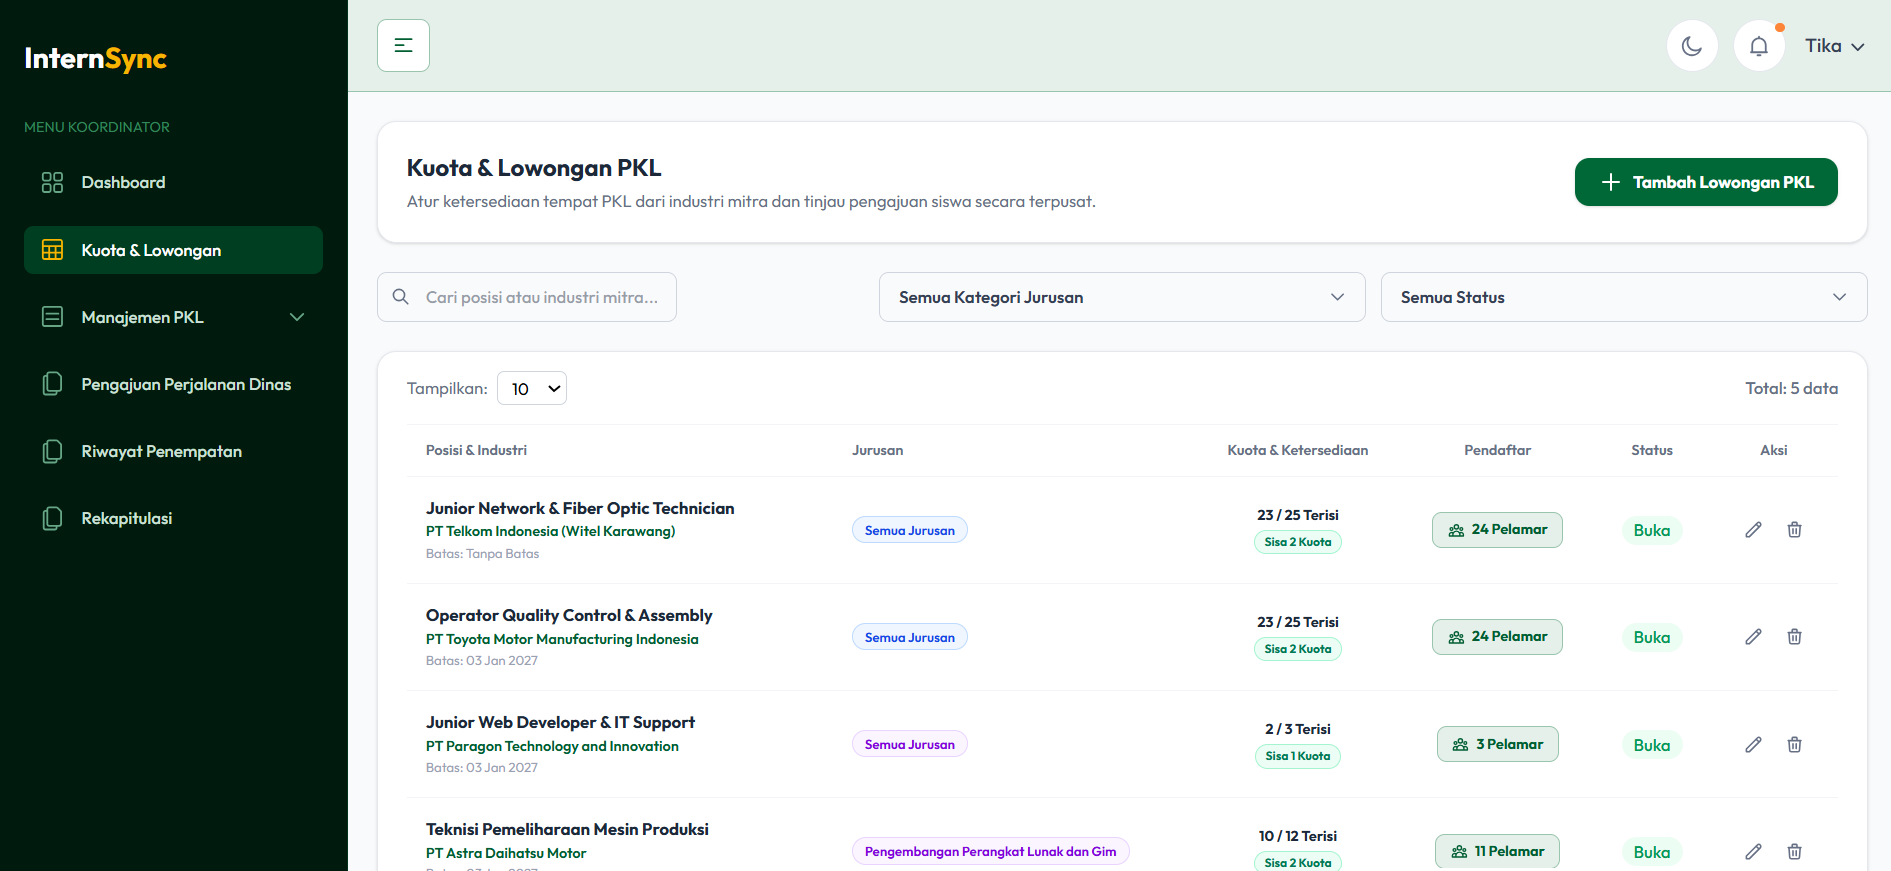
\includegraphics[width=14.00cm,height=0.78\textheight,keepaspectratio]{gambar/gambar-3-14.png}
\caption{Antarmuka Manajemen Lowongan PKL (Koordinator)}\label{fig:3.14}
\end{figure}

Halaman ini digunakan oleh Koordinator PKL untuk merumuskan dan mengelola lowongan magang berdasarkan daftar industri mitra yang telah disahkan oleh pihak Hubin. Antarmuka berbentuk data table dengan tombol inisiasi Tambah Lowongan. Formulir pembuatan lowongan mengintegrasikan elemen pilihan industri terikat, penentuan posisi pekerjaan (job role), kualifikasi keahlian yang disyaratkan, kuota kapasitas siswa yang dapat diterima, batas akhir pendaftaran (deadline), serta penentuan klasifikasi lowongan (lowongan umum untuk seluruh kompetensi keahlian atau lowongan khusus yang dibatasi untuk jurusan spesifik). Kolom aksi menyediakan opsi untuk mengubah rincian lowongan atau menutup status pendaftaran secara real-time.

\begin{figure}[H]
\centering
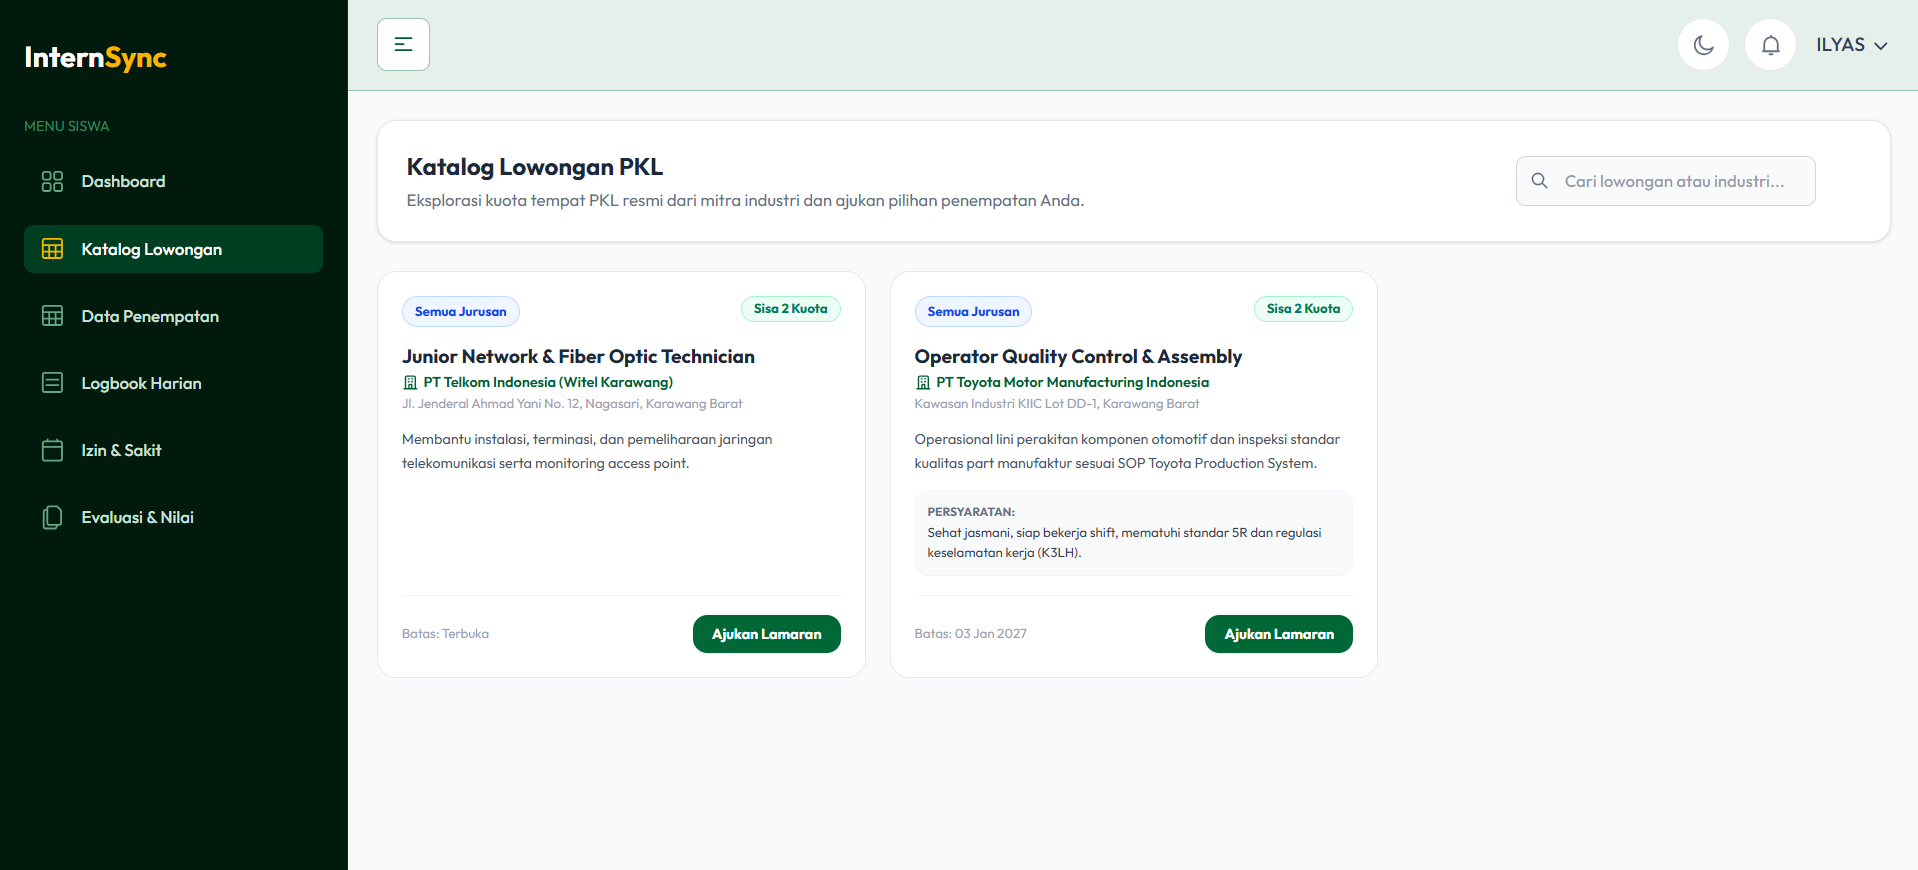
\includegraphics[width=14.00cm,height=0.78\textheight,keepaspectratio]{gambar/gambar-3-15.png}
\caption{Antarmuka Katalog dan Pendaftaran Lowongan PKL (Siswa)}\label{fig:3.15}
\end{figure}

Antarmuka ini menyajikan informasi seluruh peluang penempatan PKL aktif kepada siswa prakerin dalam format kartu interaktif (\textit{grid cards}) yang responsif dan informatif. Setiap kartu lowongan memvisualisasikan kategori jurusan (Semua Jurusan atau jurusan spesifik), indikator sisa kuota yang tersedia, judul posisi pekerjaan, nama dan alamat industri mitra, deskripsi tugas, kotak persyaratan khusus (seperti kepatuhan K3LH), serta batas waktu pendaftaran. Siswa dapat mencari lowongan melalui kolom pencarian di sudut kanan atas dan langsung mengajukan pendaftaran mandiri dengan menekan tombol Ajukan Lamaran pada kartu lowongan yang diminati. Sistem menyematkan validasi otomatis; tombol lamaran dinonaktifkan apabila kuota telah terisi penuh atau siswa telah berstatus aktif menjalani PKL.

\begin{figure}[H]
\centering
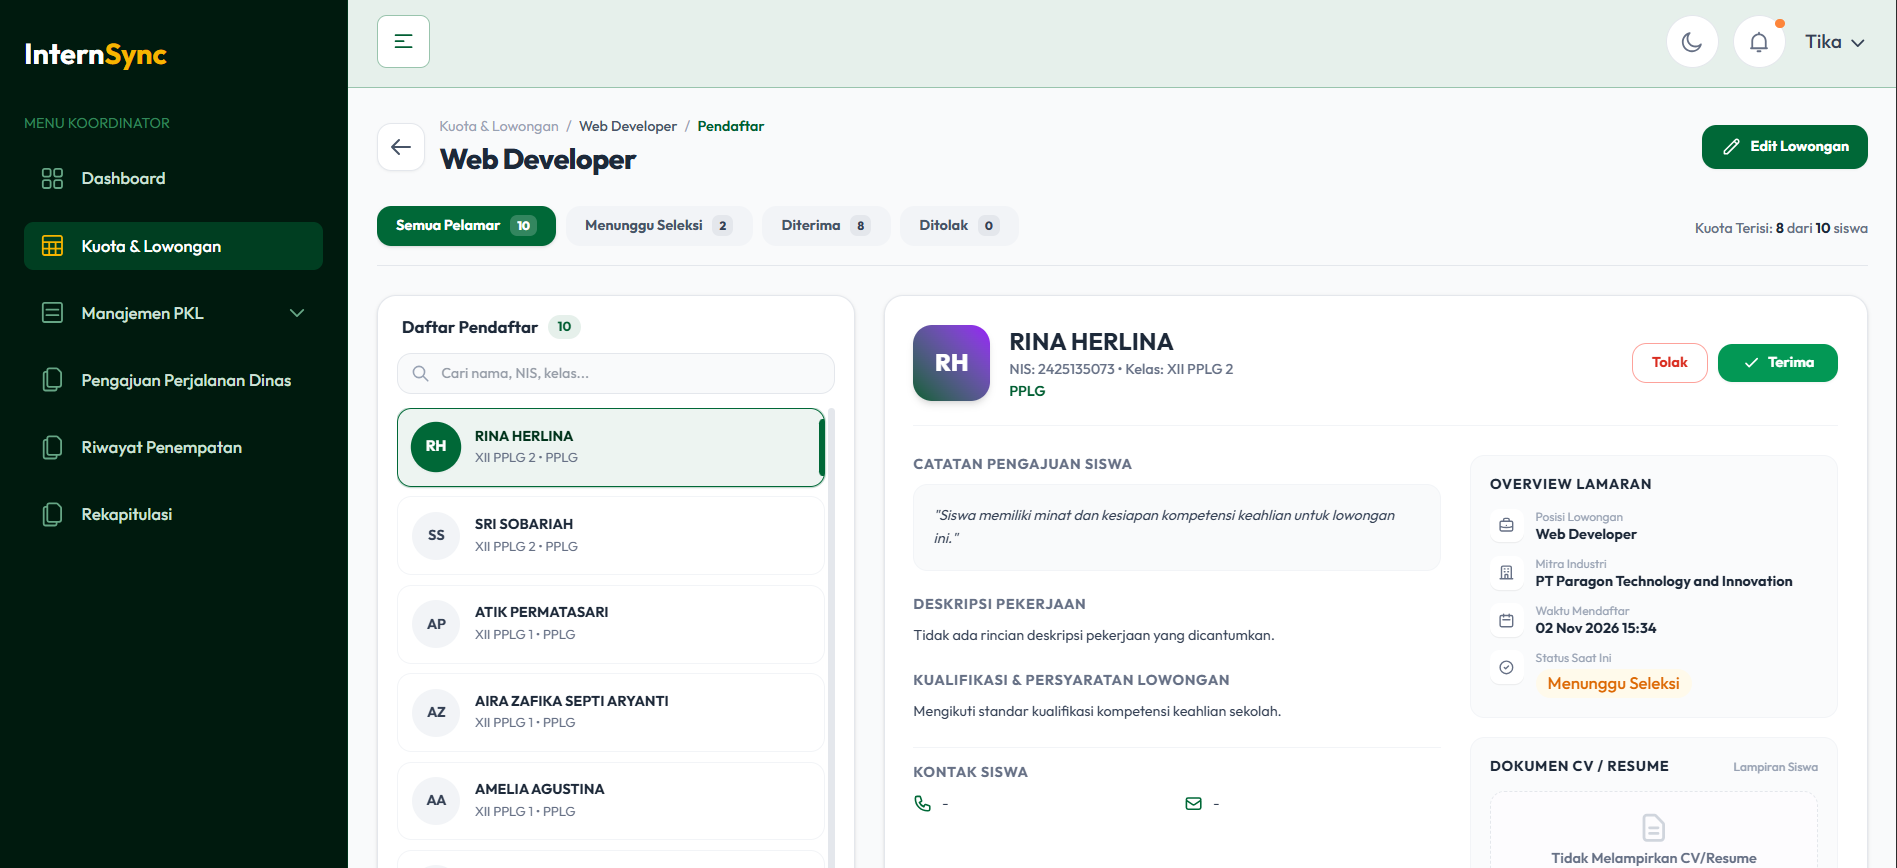
\includegraphics[width=14.00cm,height=0.78\textheight,keepaspectratio]{gambar/gambar-3-16.png}
\caption{Antarmuka Seleksi Pendaftar Lowongan (Koordinator)}\label{fig:3.16}
\end{figure}

Halaman ini merupakan decision support interface bagi Koordinator PKL untuk memverifikasi dan menyortir berkas permohonan siswa yang mendaftar pada setiap entitas lowongan. Antarmuka menyajikan daftar nominatif siswa pelamar yang dilengkapi metrik jurusan, kelas, dan tanggal pengajuan. Pada kolom aksi, Koordinator diberikan otoritas seleksi melalui tombol Terima atau Tolak disertai modal input catatan alasan penolakan. Data siswa yang dinyatakan diterima pada antarmuka ini secara otomatis terkonsolidasi menjadi data kandidat definitif untuk diproses ke dalam tahap penyusunan pengajuan penempatan PKL resmi.

\begin{figure}[H]
\centering
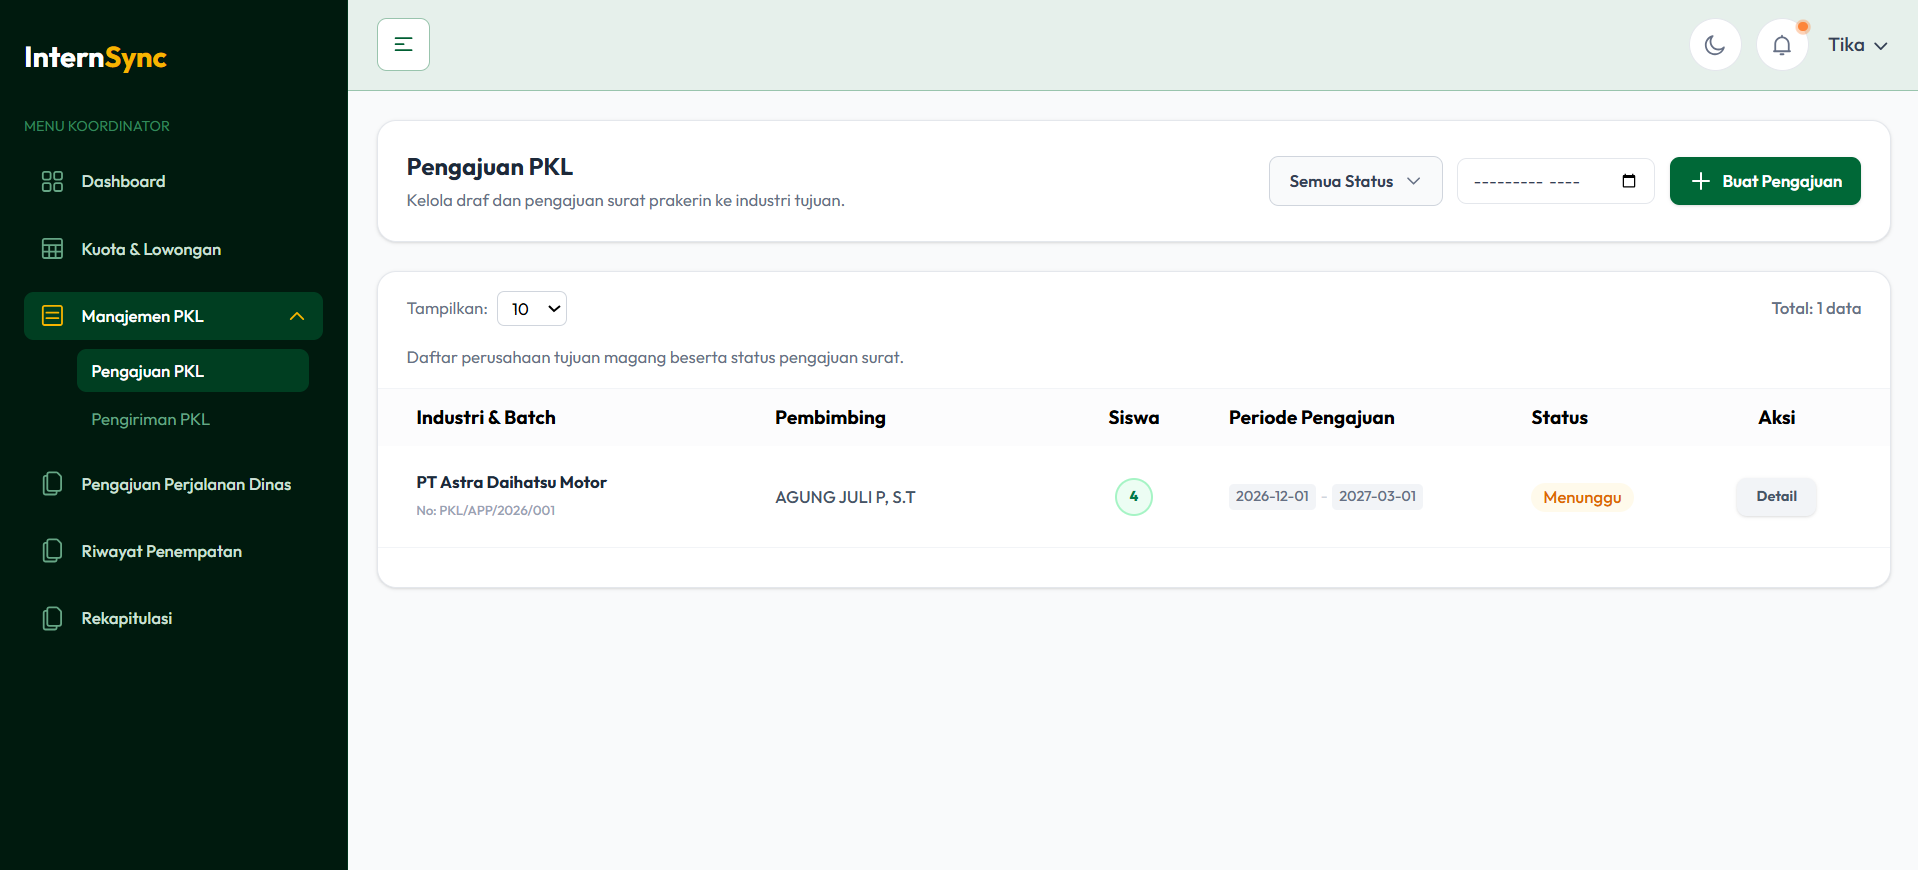
\includegraphics[width=14.00cm,height=0.78\textheight,keepaspectratio]{gambar/gambar-3-17.png}
\caption{Antarmuka Manajemen Pengajuan PKL (Koordinator)}\label{fig:3.17}
\end{figure}

Halaman ini merupakan antarmuka manajemen dokumen pengajuan penempatan PKL yang dikelola oleh Koordinator PKL pada submenu Pengajuan PKL. Komponen utama menampilkan \textit{data table} daftar permohonan penempatan yang telah disusun berdasarkan hasil seleksi lowongan, memuat atribut nama Industri dan Batch (beserta nomor registrasi dokumen \texttt{PKL/APP/...}), nama Guru Pembimbing yang ditugaskan, jumlah siswa dalam \textit{batch}, periode pengajuan magang, serta \textit{badge} status persetujuan (Menunggu, Disetujui, atau Ditolak). Halaman ini dilengkapi filter status dan periode tanggal, tombol Detail untuk meninjau rincian nominatif siswa, serta tombol + Buat Pengajuan di sudut kanan atas untuk membuka formulir pengajuan penempatan yang diteruskan kepada Waka Hubin.

\begin{figure}[H]
\centering
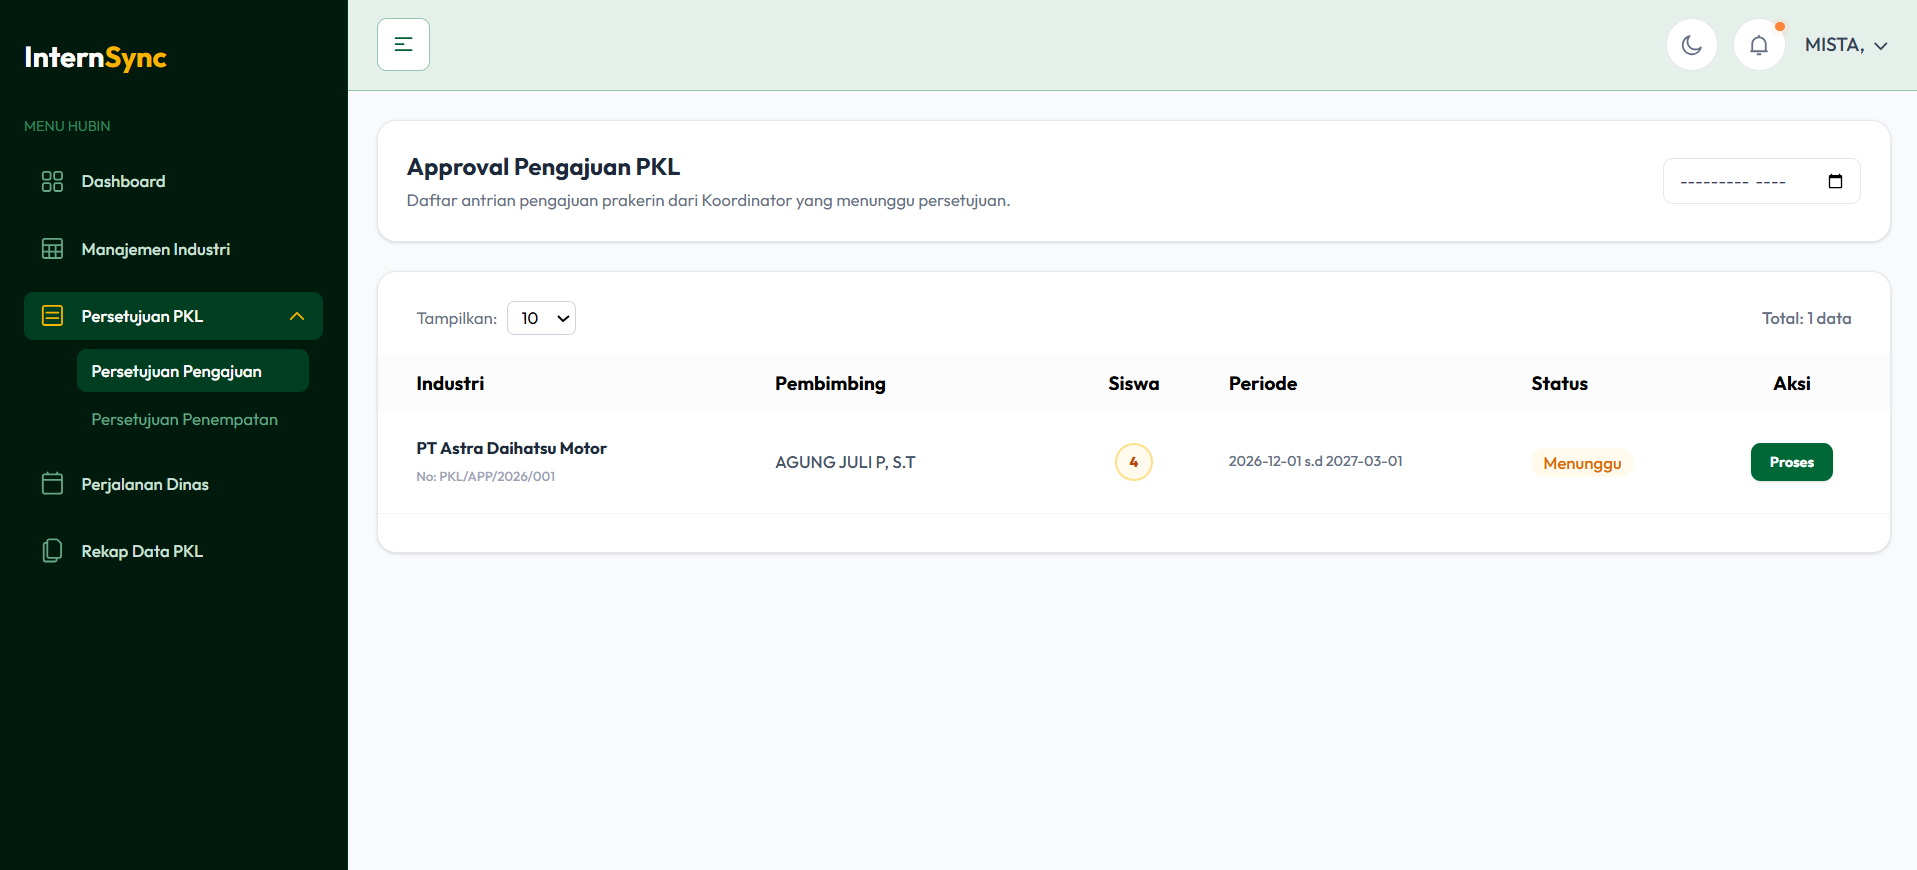
\includegraphics[width=14.00cm,height=0.78\textheight,keepaspectratio]{gambar/gambar-3-18.png}
\caption{Antarmuka Evaluasi dan Persetujuan Pengajuan PKL (Hubin)}\label{fig:3.18}
\end{figure}

Antarmuka ini berfungsi sebagai halaman antrean persetujuan (\textit{approval queue}) dokumen pengajuan penempatan PKL bagi Waka Hubin pada submenu Persetujuan Pengajuan. Halaman ini menyajikan \textit{data table} seluruh pengajuan masuk dari Koordinator PKL yang berstatus Menunggu, mencakup informasi perusahaan tujuan beserta nomor surat pengajuan, nama guru pembimbing pendamping, jumlah siswa peserta, serta rentang periode pelaksanaan yang diusulkan. Pada kolom aksi tersedia tombol Proses untuk membuka rincian dokumen dan memberikan keputusan persetujuan, yang otomatis menerbitkan Surat Pengantar PKL berformat PDF, atau penolakan disertai alasan revisi.

\begin{figure}[H]
\centering
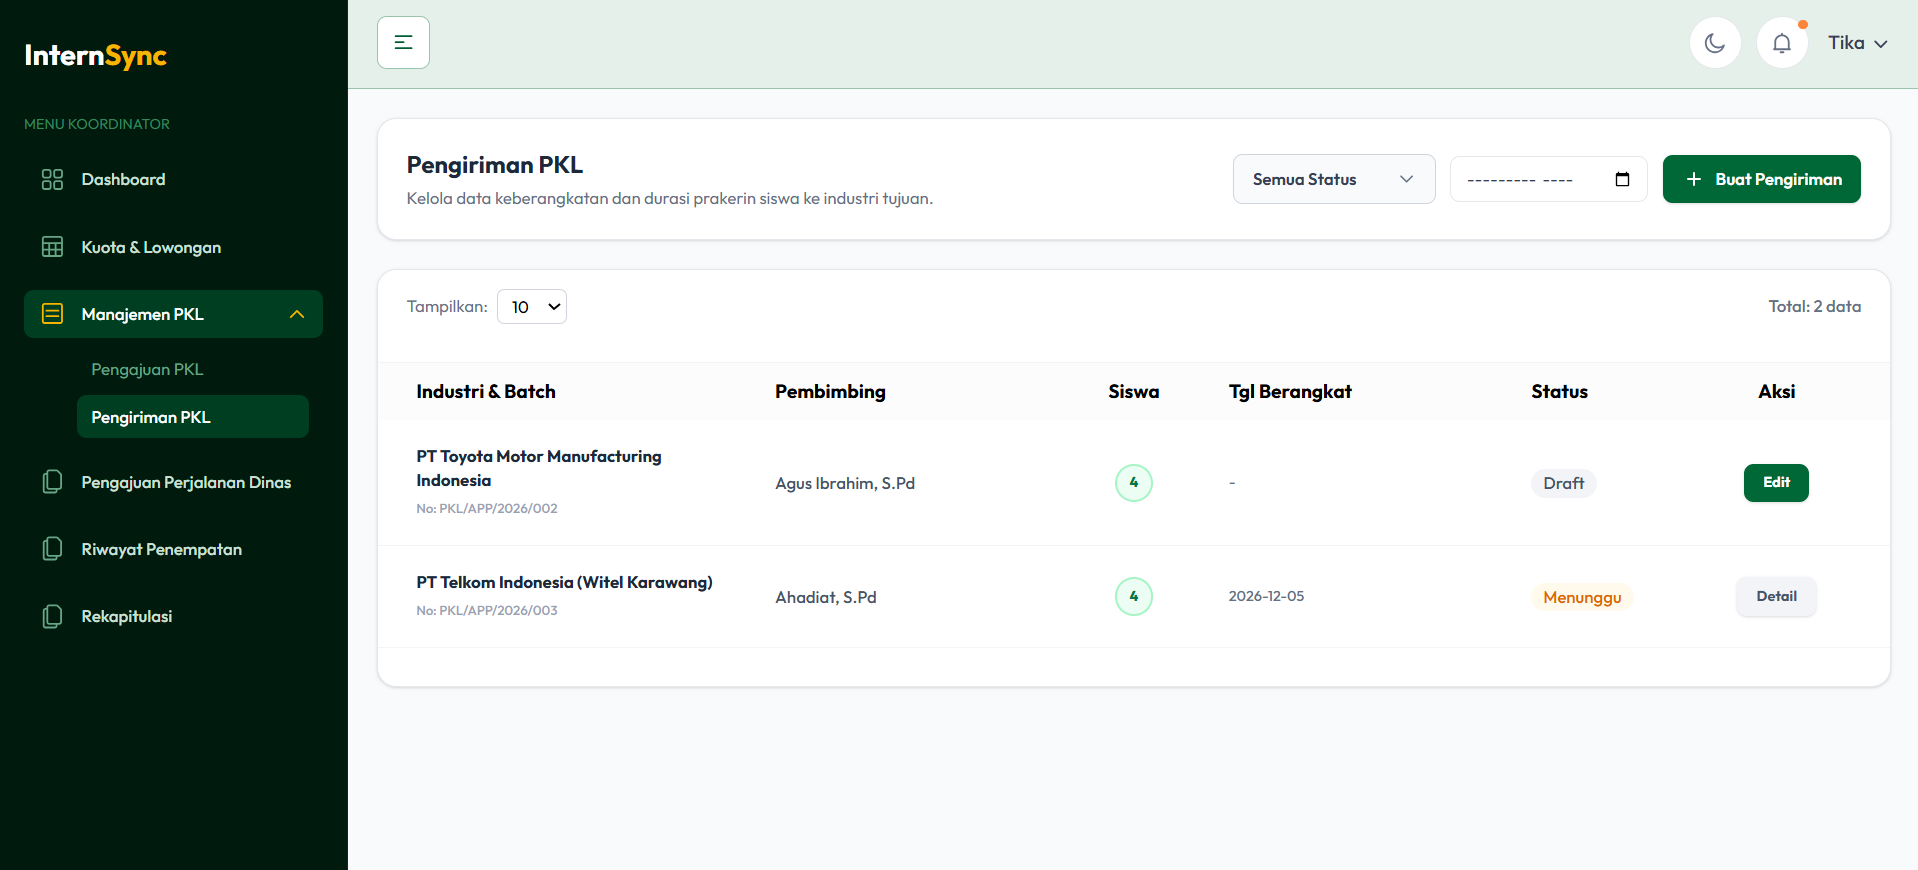
\includegraphics[width=14.00cm,height=0.78\textheight,keepaspectratio]{gambar/gambar-3-19.png}
\caption{Antarmuka Proses Pengiriman dan Penetapan Durasi PKL (Koordinator)}\label{fig:3.19}
\end{figure}

Halaman ini merupakan tindak lanjut pada submenu Pengiriman PKL setelah dokumen pengajuan awal disetujui Waka Hubin, yang berfokus pada pengelolaan jadwal keberangkatan siswa ke industri. Antarmuka menyajikan \textit{data table} daftar pengiriman per \textit{batch} industri beserta nama guru pembimbing, jumlah siswa, tanggal keberangkatan definitif, dan \textit{badge} status pengiriman (Draft atau Menunggu). Koordinator dapat menekan tombol + Buat Pengiriman atau Edit pada baris berstatus Draft untuk menetapkan tanggal mulai dan durasi PKL (3 atau 6 bulan), atau menekan Detail untuk memantau pengiriman yang menunggu \textit{clearance} akhir Hubin.

\begin{figure}[H]
\centering
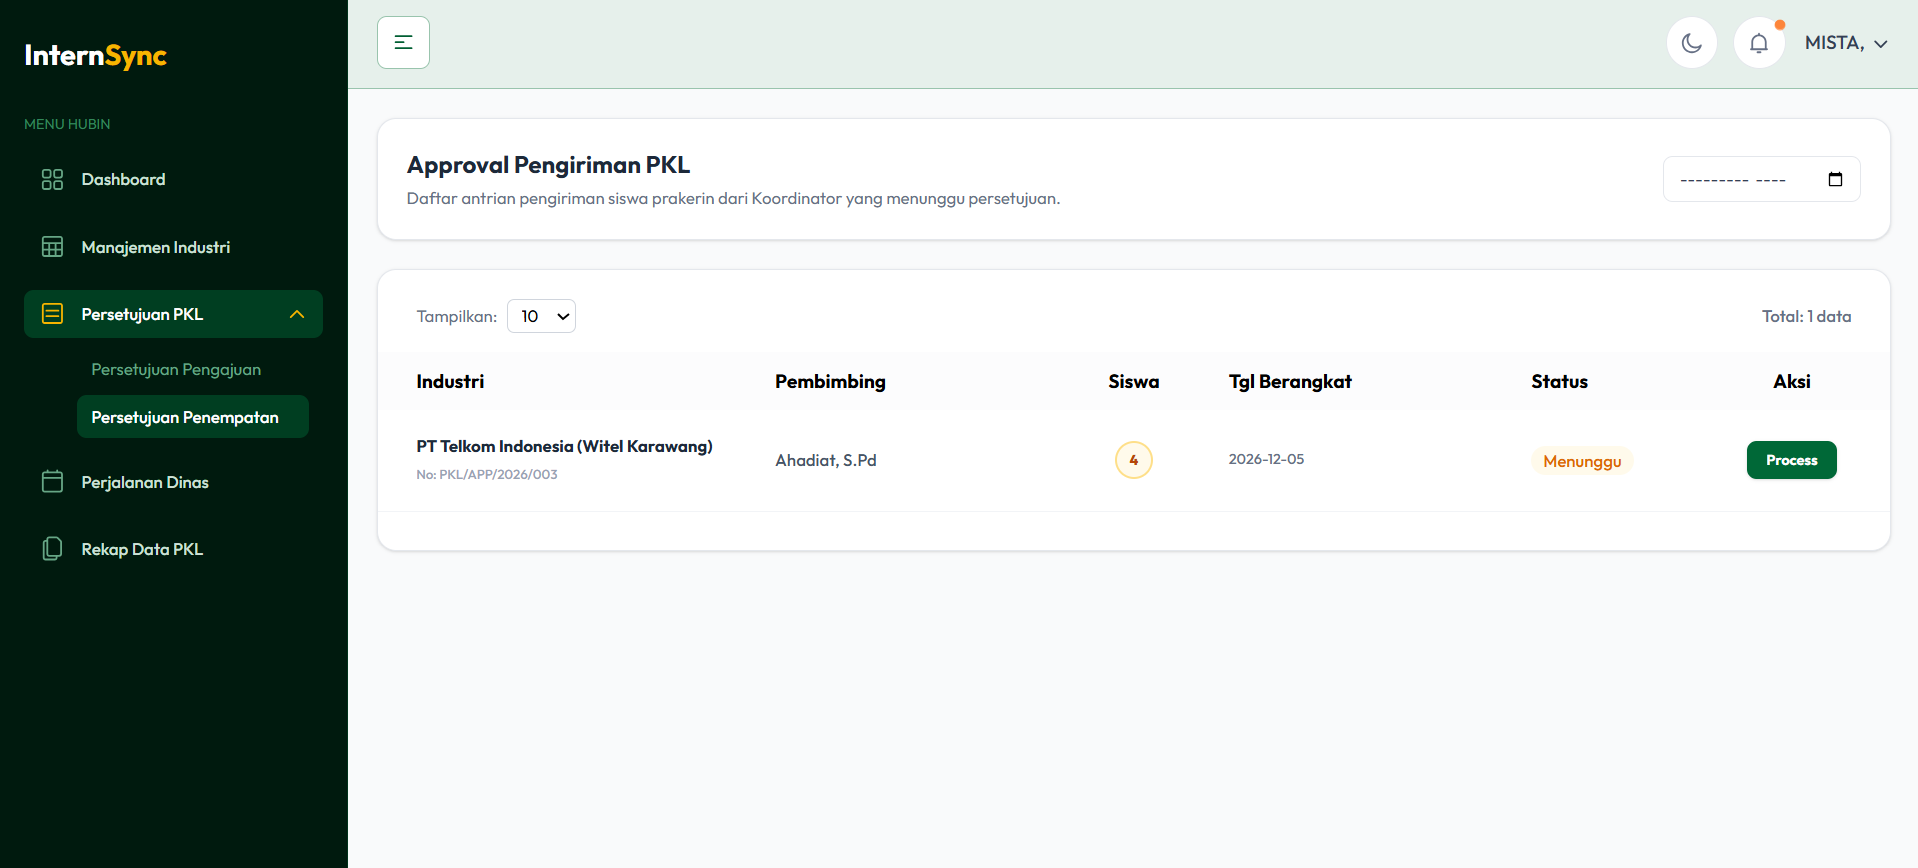
\includegraphics[width=14.00cm,height=0.78\textheight,keepaspectratio]{gambar/gambar-3-20.png}
\caption{Antarmuka Final Clearance dan Persetujuan Penempatan PKL (Hubin)}\label{fig:3.20}
\end{figure}

Antarmuka ini merepresentasikan tahap validasi keberangkatan akhir (\textit{final clearance}) oleh Waka Hubin pada submenu Persetujuan Penempatan sebelum siswa resmi berstatus aktif melaksanakan PKL di industri. Halaman ini menampilkan \textit{data table} antrean pengiriman siswa dari Koordinator PKL yang memuat informasi industri tujuan dan nomor dokumen, guru pembimbing, jumlah siswa, tanggal keberangkatan, serta status Menunggu. Melalui tombol Process, Waka Hubin dapat meninjau rincian final dan mengesahkan keberangkatan tersebut. Pengesahan menjadi pemicu sistemik yang mengubah status siswa menjadi aktif pada tabel \texttt{tr\_internships} serta membuka akses ke modul operasional harian (\textit{logbook} dan perizinan).

\subsubsection{Fase Pelaksanaan PKL (Monitoring, Logbook, Perizinan, dan Kunjungan)}

Fase ini memfasilitasi aktivitas operasional harian selama masa magang berlangsung, mencakup pencatatan rekam aktivitas kerja siswa, tata kelola presensi dan perizinan, verifikasi berkala oleh guru pembimbing, serta pemantauan kunjungan supervisi ke industri.

\begin{figure}[H]
\centering
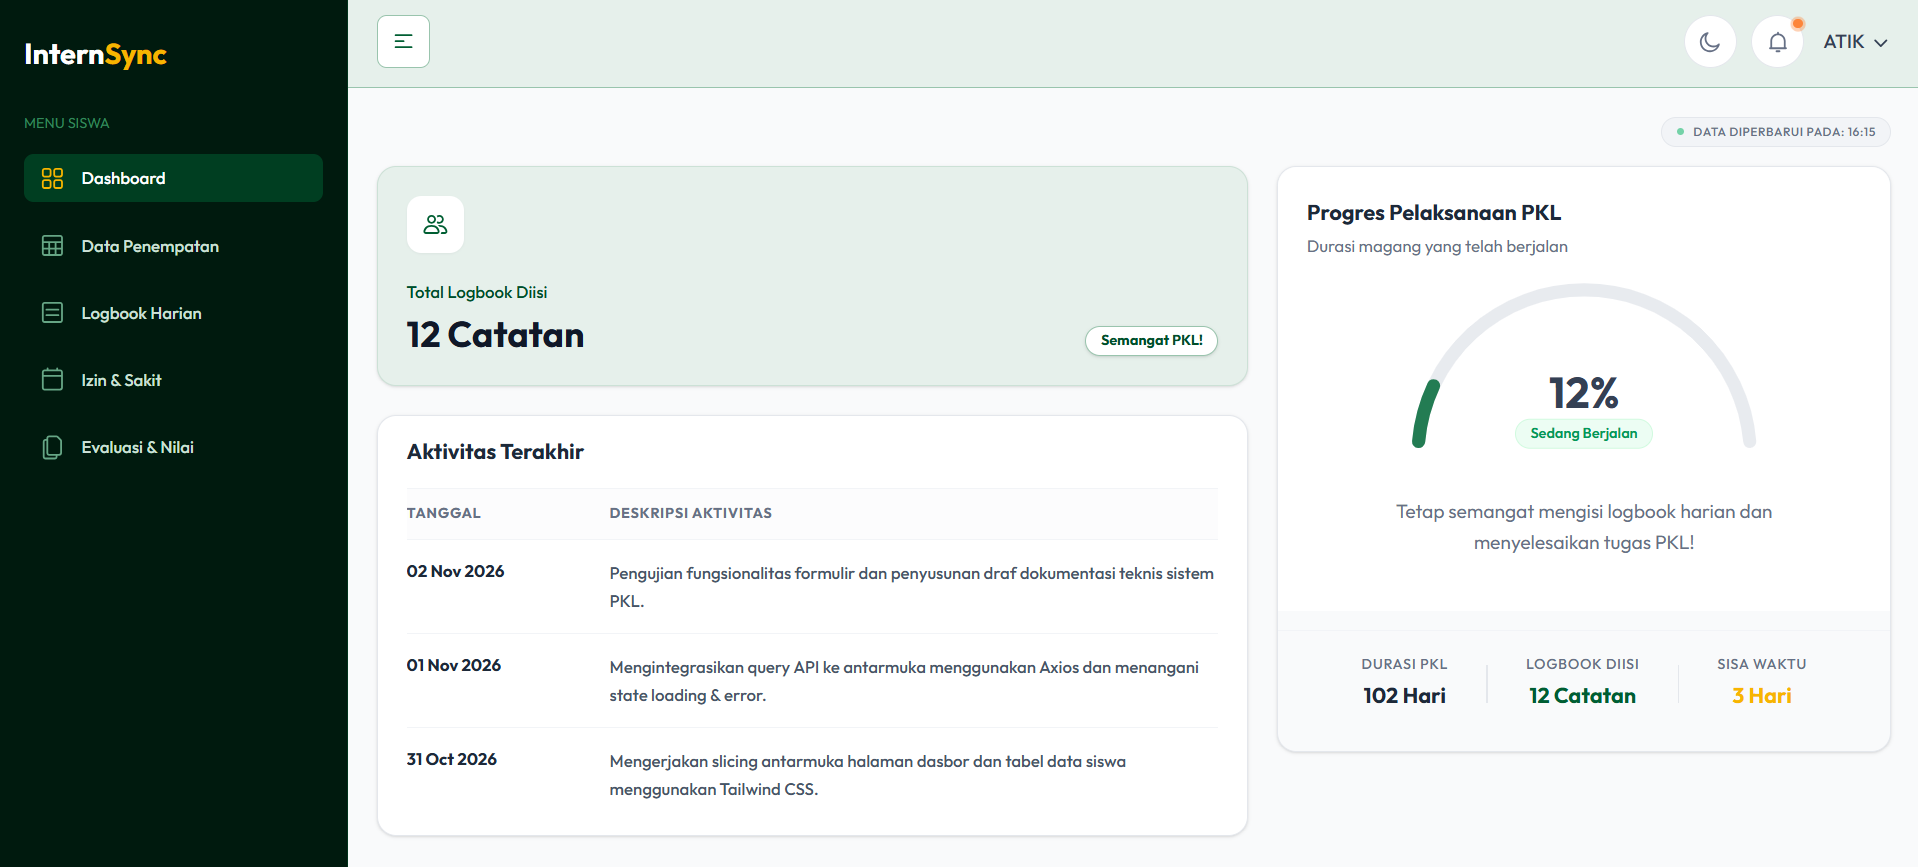
\includegraphics[width=14.00cm,height=0.78\textheight,keepaspectratio]{gambar/gambar-3-21.png}
\caption{Dasbor Antarmuka Siswa Prakerin (Tracking Progres PKL)}\label{fig:3.21}
\end{figure}

Antarmuka dasbor siswa berfungsi sebagai pusat kendali dan pemantauan informasi personal siswa selama menjalani masa PKL. Pada sisi kiri atas terdapat kartu ringkasan kuantitatif yang menampilkan metrik Total Logbook Diisi beserta lencana motivasi pelaksanaan. Di bawahnya tersaji tabel linimasa Aktivitas Terakhir yang merangkum tanggal dan deskripsi kegiatan \textit{logbook} terbaru. Pada sisi kanan, dasbor menampilkan \textit{gauge chart} (grafik setengah lingkaran progresif) pada panel Progres Pelaksanaan PKL yang menghitung persentase waktu magang yang telah ditempuh beserta total durasi PKL (hari), jumlah \textit{logbook} diisi, dan sisa waktu pelaksanaan.

\begin{figure}[H]
\centering
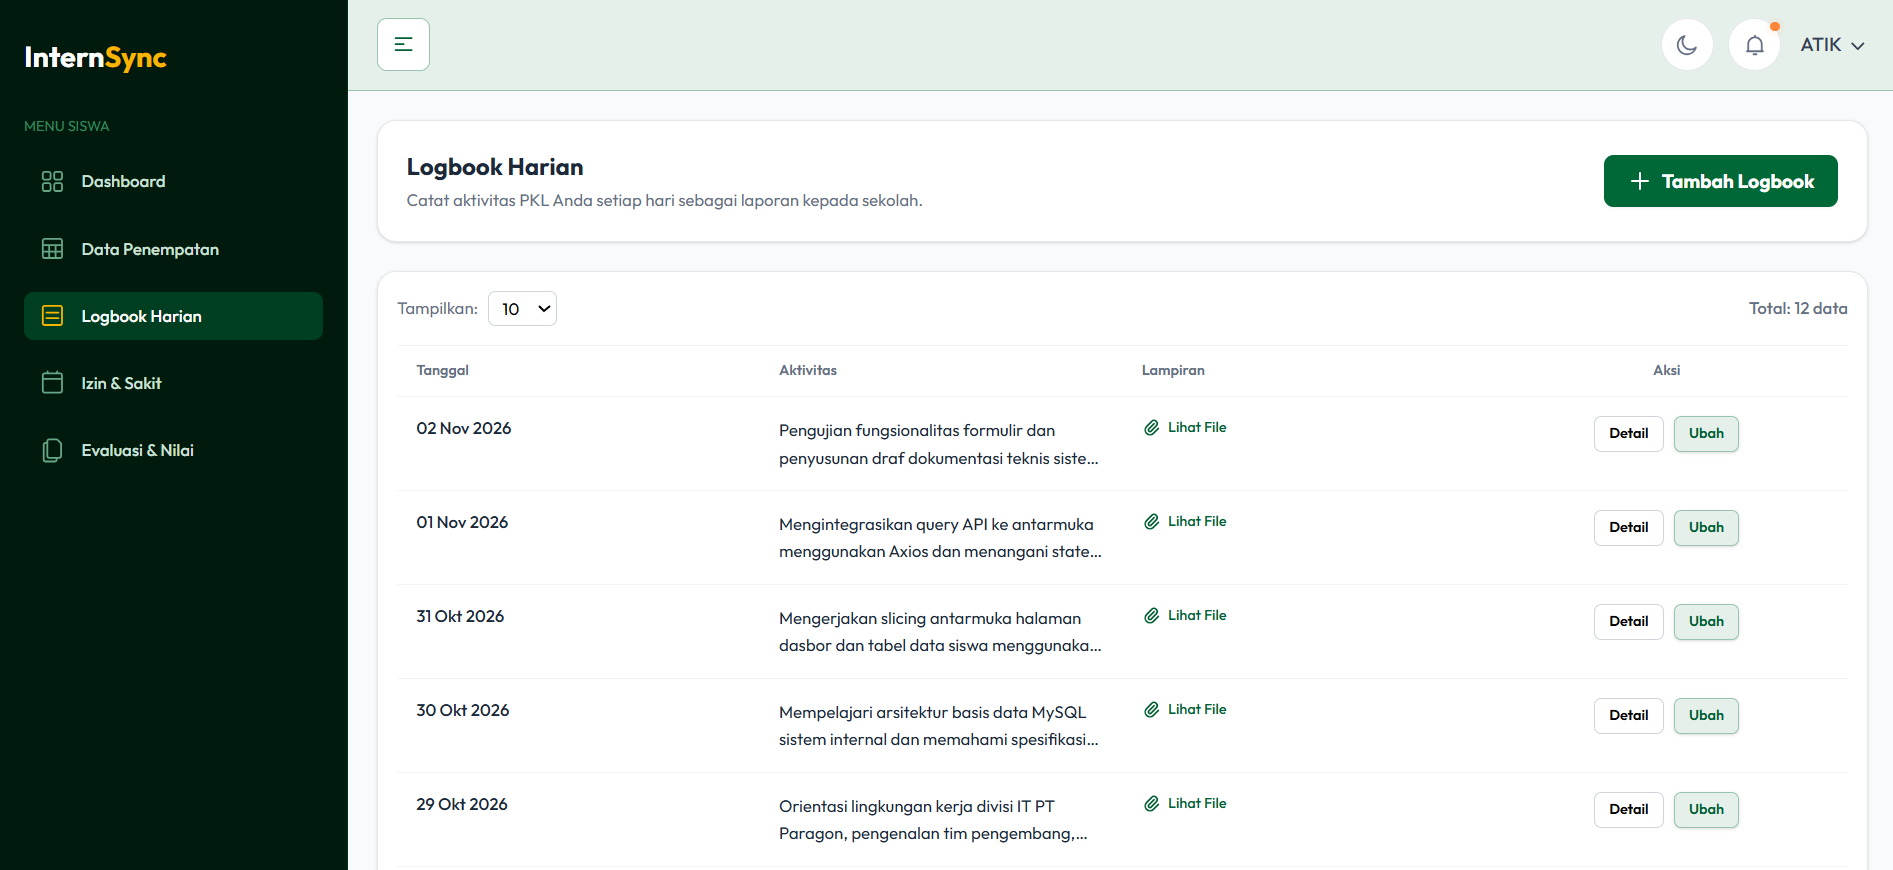
\includegraphics[width=14.00cm,height=0.78\textheight,keepaspectratio]{gambar/gambar-3-22.png}
\caption{Antarmuka Manajemen dan Pengisian Logbook Harian Siswa}\label{fig:3.22}
\end{figure}

Halaman ini merupakan instrumen utama siswa untuk mencatat rekam kegiatan operasional di industri secara mandiri (self-reporting logbook). Sistem menerapkan pendekatan pencatatan langsung tanpa melalui proses validasi berjenjang atau status persetujuan harian dari pembimbing, sehingga mempermudah siswa mendokumentasikan rutinitas kerja teknis di industri tanpa hambatan birokrasi harian. Komponen antarmuka terdiri atas data table rekapitulasi logbook per tanggal yang memuat kolom Tanggal pelaksanaan, Aktivitas pekerjaan, Lampiran bukti fisik, serta kolom Aksi. Tombol + Tambah Logbook membuka modal formulir pengisian tanggal kegiatan, uraian teknis pekerjaan yang dilakukan, serta tombol unggah berkas bukti fisik (foto kegiatan atau dokumen kerja). Formulir ini dilengkapi validasi otomatis berbasis kalender kerja yang membatasi pengisian hanya saat status PKL aktif, mendeteksi tanggal kerja yang belum diisi (mengecualikan hari libur dan izin/sakit), serta mencegah duplikasi pencatatan pada tanggal yang sama. Pada kolom aksi, siswa dapat menekan tombol Detail untuk meninjau rincian catatan aktivitas atau tombol Ubah untuk melakukan pembaruan konten dan lampiran kegiatan secara fleksibel.

\begin{figure}[H]
\centering
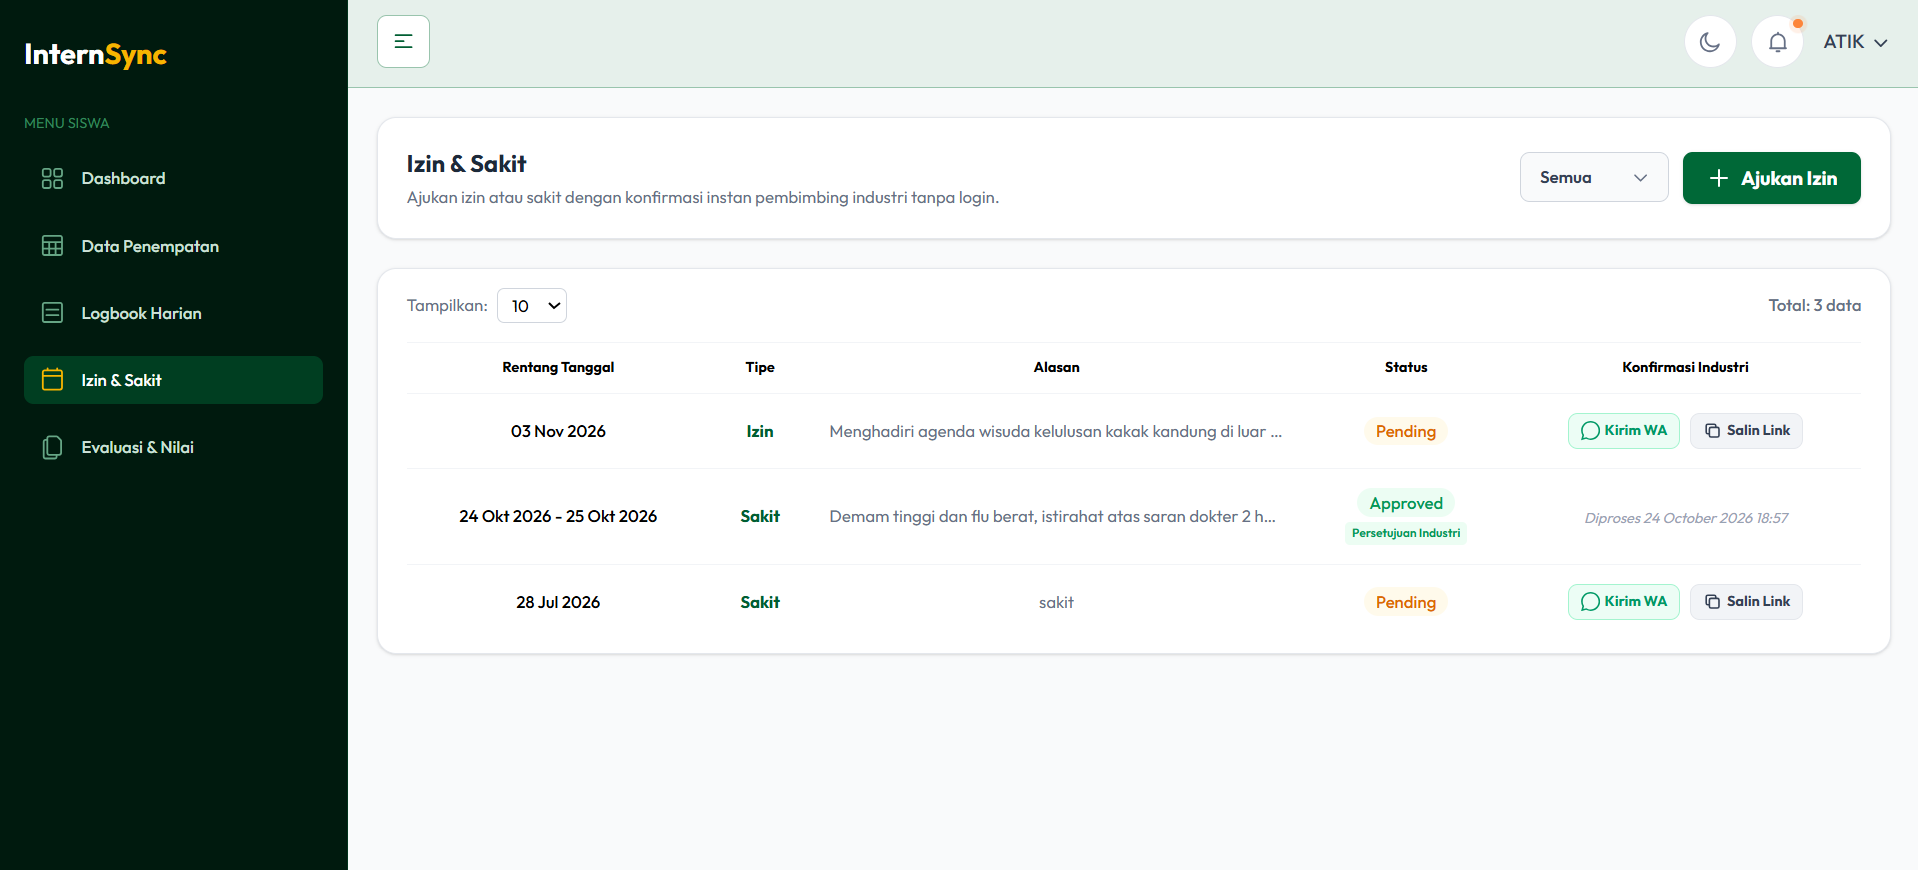
\includegraphics[width=14.00cm,height=0.78\textheight,keepaspectratio]{gambar/gambar-3-23.png}
\caption{Antarmuka Pengajuan Izin dan Sakit Siswa}\label{fig:3.23}
\end{figure}

Antarmuka ini menyediakan pencatatan ketidakhadiran siswa secara tertib dan transparan. Komponen utama menampilkan \textit{data table} riwayat permohonan izin/sakit dengan kolom Rentang Tanggal, Tipe permohonan (Izin atau Sakit), Alasan, \textit{badge} Status (Pending atau Approved beserta keterangan Persetujuan Industri), serta kolom Konfirmasi Industri. Siswa dapat menekan tombol + Ajukan Izin untuk menginput tanggal, alasan, dan mengunggah bukti sah (surat dokter atau surat orang tua). Untuk permohonan Pending, tersedia tombol Kirim WA dan Salin Link agar siswa dapat meneruskan tautan token persetujuan unik kepada Pembimbing Industri tanpa login.

\begin{figure}[H]
\centering
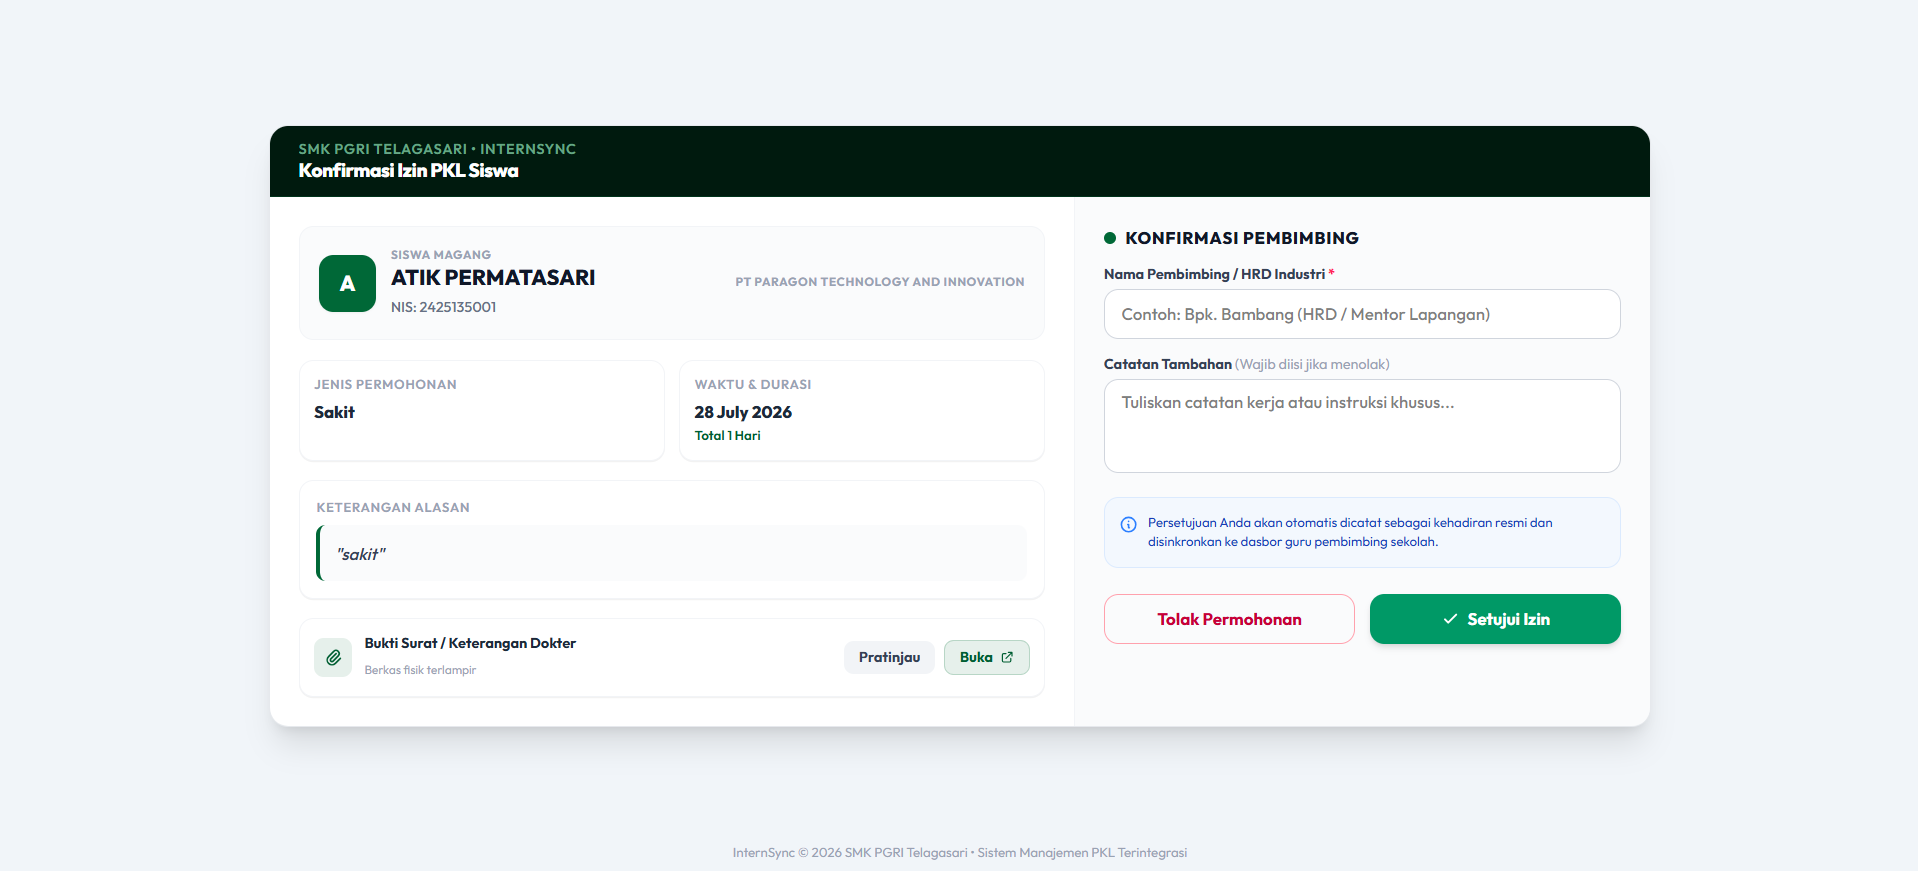
\includegraphics[width=14.00cm,height=0.78\textheight,keepaspectratio]{gambar/gambar-3-24.png}
\caption{Antarmuka Web Publik Persetujuan Izin Siswa via Tautan Token (Pembimbing Industri)}\label{fig:3.24}
\end{figure}

Halaman ini merupakan antarmuka publik berbasis rute token aman (/approval/izin/:token) yang digunakan Pembimbing Industri untuk memvalidasi permohonan izin siswa tanpa perlu login ke sistem. Halaman web responsif ini menampilkan rincian data siswa, tanggal ketidakhadiran, alasan, serta pratinjau dokumen surat dokter pendukung. Pembimbing Industri dapat menekan tombol Setujui Izin atau Tolak Izin. Sistem juga menerapkan mekanisme fallback 24 jam: apabila Pembimbing Industri belum merespons dalam kurun waktu tersebut, wewenang verifikasi izin dialihkan ke Guru Pembimbing Sekolah guna mencegah stagnasi data presensi.

\begin{figure}[H]
\centering
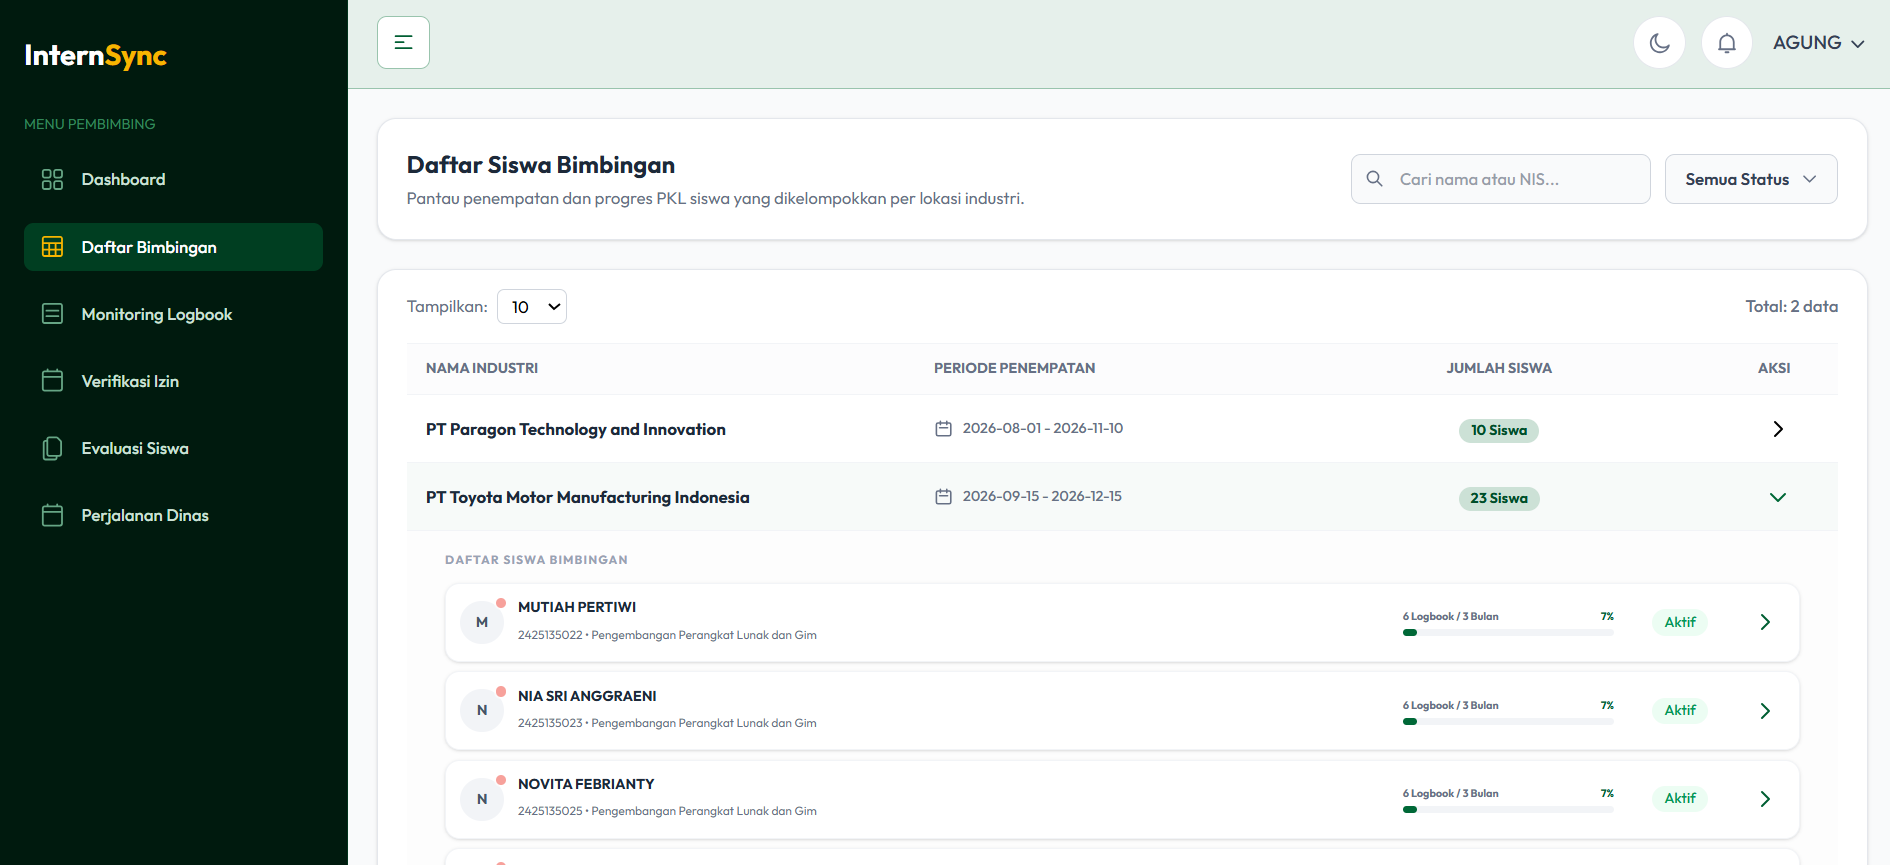
\includegraphics[width=14.00cm,height=0.78\textheight,keepaspectratio]{gambar/gambar-3-25.png}
\caption{Antarmuka Daftar Siswa Bimbingan (Guru Pembimbing)}\label{fig:3.25}
\end{figure}

Halaman pembimbing ini menyajikan informasi pengawasan siswa yang berada di bawah tanggung jawab supervisinya. Antarmuka menampilkan tabel hierarkis yang mengelompokkan siswa berdasarkan industri tempat mereka ditempatkan. Setiap baris data siswa memuat indikator progres pengisian logbook, status operasional, serta tombol aksi untuk meninjau detail logbook, riwayat perizinan, dan agenda kunjungan.

\begin{figure}[H]
\centering
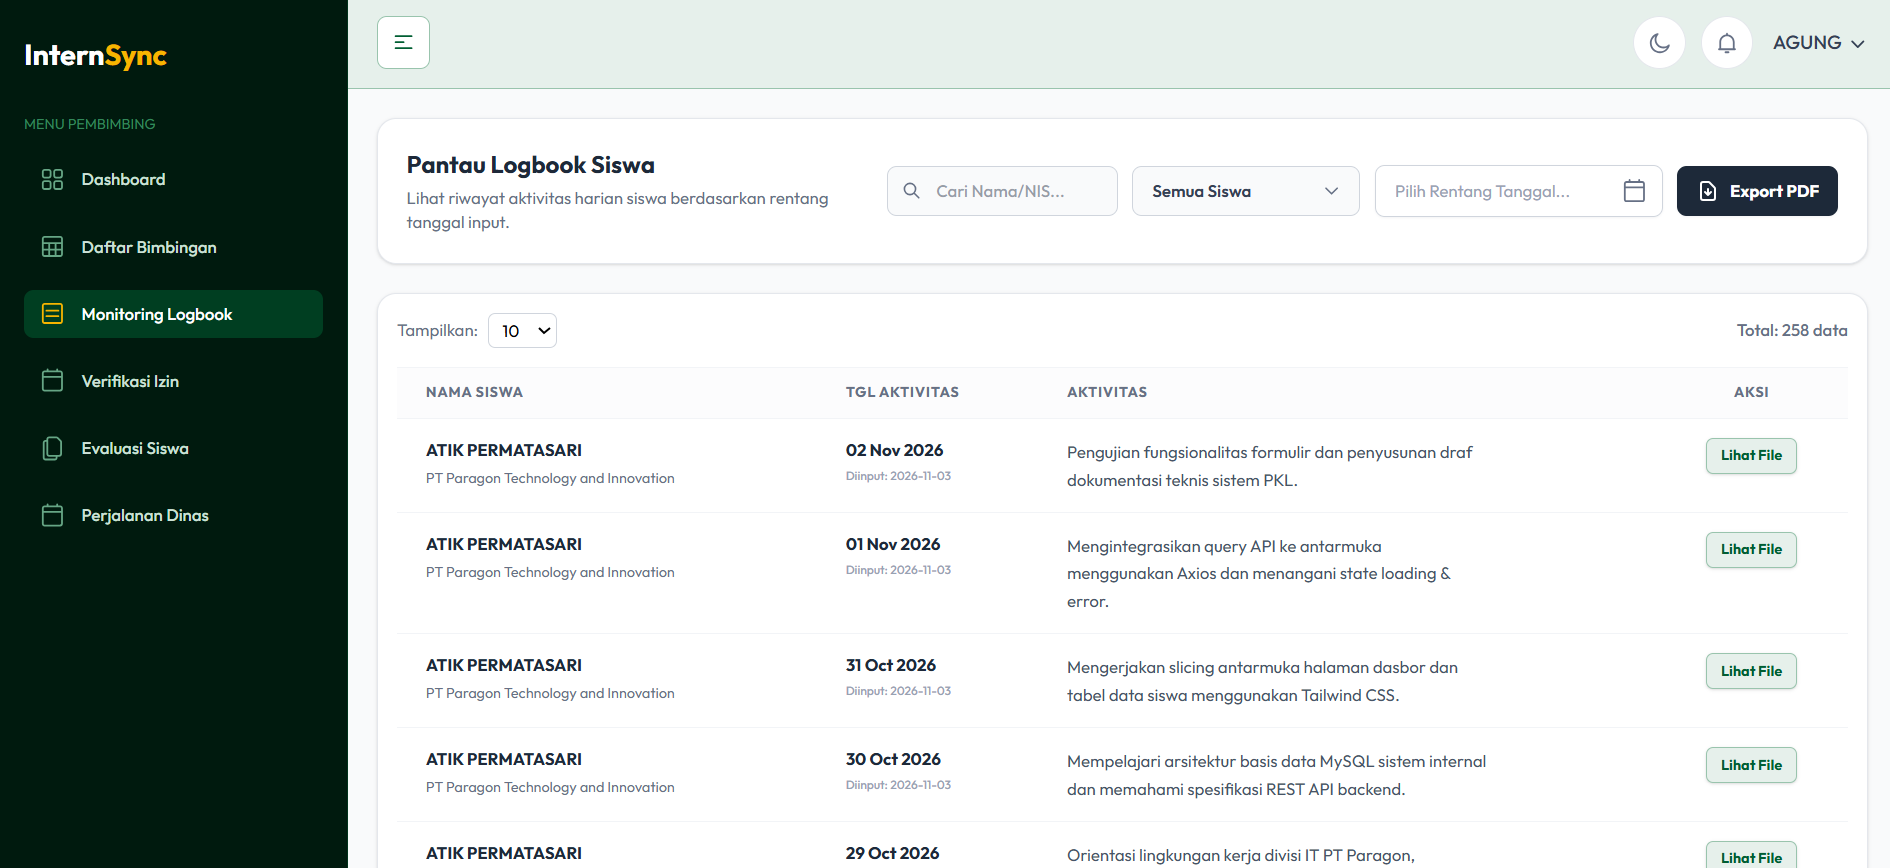
\includegraphics[width=14.00cm,height=0.78\textheight,keepaspectratio]{gambar/gambar-3-26.png}
\caption{Antarmuka Monitoring Logbook Siswa (Guru Pembimbing)}\label{fig:3.26}
\end{figure}

Antarmuka ini merupakan instrumen supervisi, pemantauan, dan kendali mutu kegiatan bimbingan magang siswa oleh guru pembimbing sekolah. Komponen utama terdiri atas data table rekapitulasi jurnal harian dengan fungsionalitas penyaringan tingkat lanjut (pencarian nama/NIS siswa, filter dropdown daftar siswa bimbingan, dan rentang tanggal kegiatan). Guru pembimbing dapat memantau kedisiplinan dan kontinuitas pengisian jurnal kerja, meninjau deskripsi aktivitas pekerjaan teknis beserta kendala yang dihadapi siswa, serta membuka berkas foto lampiran bukti fisik kegiatan secara langsung melalui modal peninjau berkas (attachment modal). Berbeda dengan pendekatan konvensional yang membebani pembimbing dengan antrean persetujuan manual per entitas baris setiap hari, sistem InternSync menerapkan mekanisme self-reporting terstruktur di mana seluruh catatan logbook yang diunggah siswa langsung terarsipkan secara transparan. Pada bagian atas tabel, halaman ini dilengkapi tombol Ekspor Logbook (PDF) yang mengompilasi seluruh catatan harian siswa secara otomatis menjadi bundel laporan resmi yang tervalidasi tanda tangan digital QR Code sebagai berkas portofolio pendukung evaluasi dan pertimbangan rubrik penilaian akhir PKL.

\begin{figure}[H]
\centering
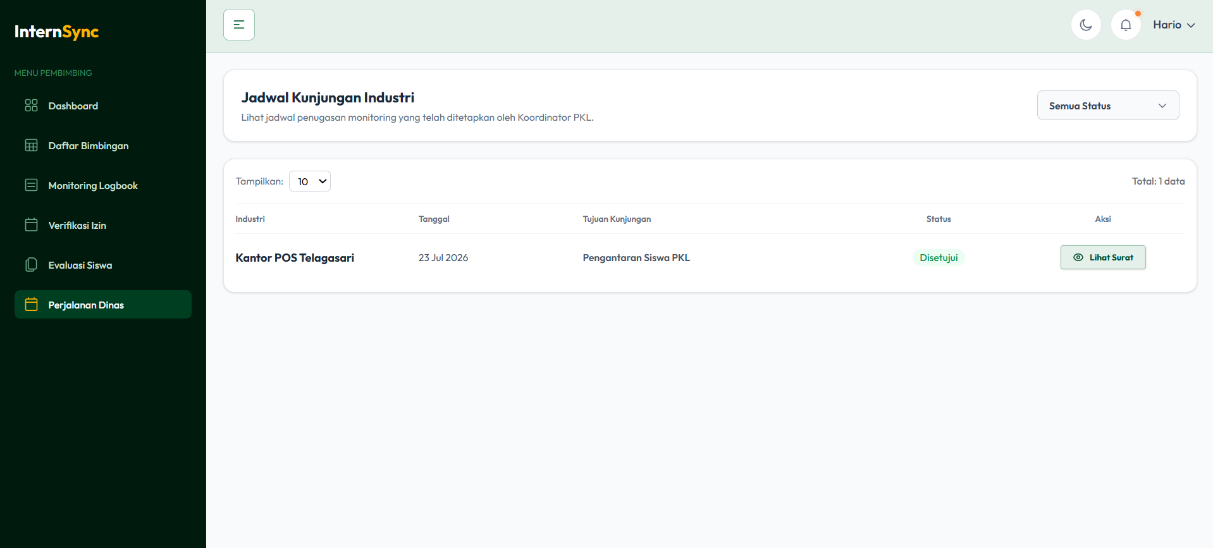
\includegraphics[width=14.00cm,height=0.78\textheight,keepaspectratio]{gambar/gambar-3-27.png}
\caption{Antarmuka Monitoring Kunjungan Industri dan Surat Tugas SPPD (Guru Pembimbing)}\label{fig:3.27}
\end{figure}

Antarmuka pada menu Perjalanan Dinas ini memfasilitasi Guru Pembimbing dalam memantau jadwal penugasan kunjungan supervisi ke industri mitra yang telah ditetapkan oleh Koordinator PKL. Komponen utama menampilkan \textit{data table} daftar penugasan kunjungan yang memuat nama industri, tanggal pelaksanaan, tujuan kunjungan (seperti pengantaran Siswa PKL), serta \textit{badge} status persetujuan (Disetujui). Pada kolom aksi tersedia tombol Lihat Surat untuk melihat dan mengunduh dokumen Surat Perintah Perjalanan Dinas (SPPD) resmi berformat PDF.

\subsubsection{Fase Pasca-PKL (Evaluasi Kinerja, Rubrik Penilaian Akhir, dan Rekapitulasi)}

Fase penutup ini mencakup alur finalisasi nilai hasil pelaksanaan PKL yang mengintegrasikan penilaian kinerja industri dan evaluasi laporan sekolah berdasarkan rubrik baku, publikasi hasil nilai kepada siswa, serta ekstraksi laporan rekapitulasi akhir sekolah.

\begin{figure}[H]
\centering
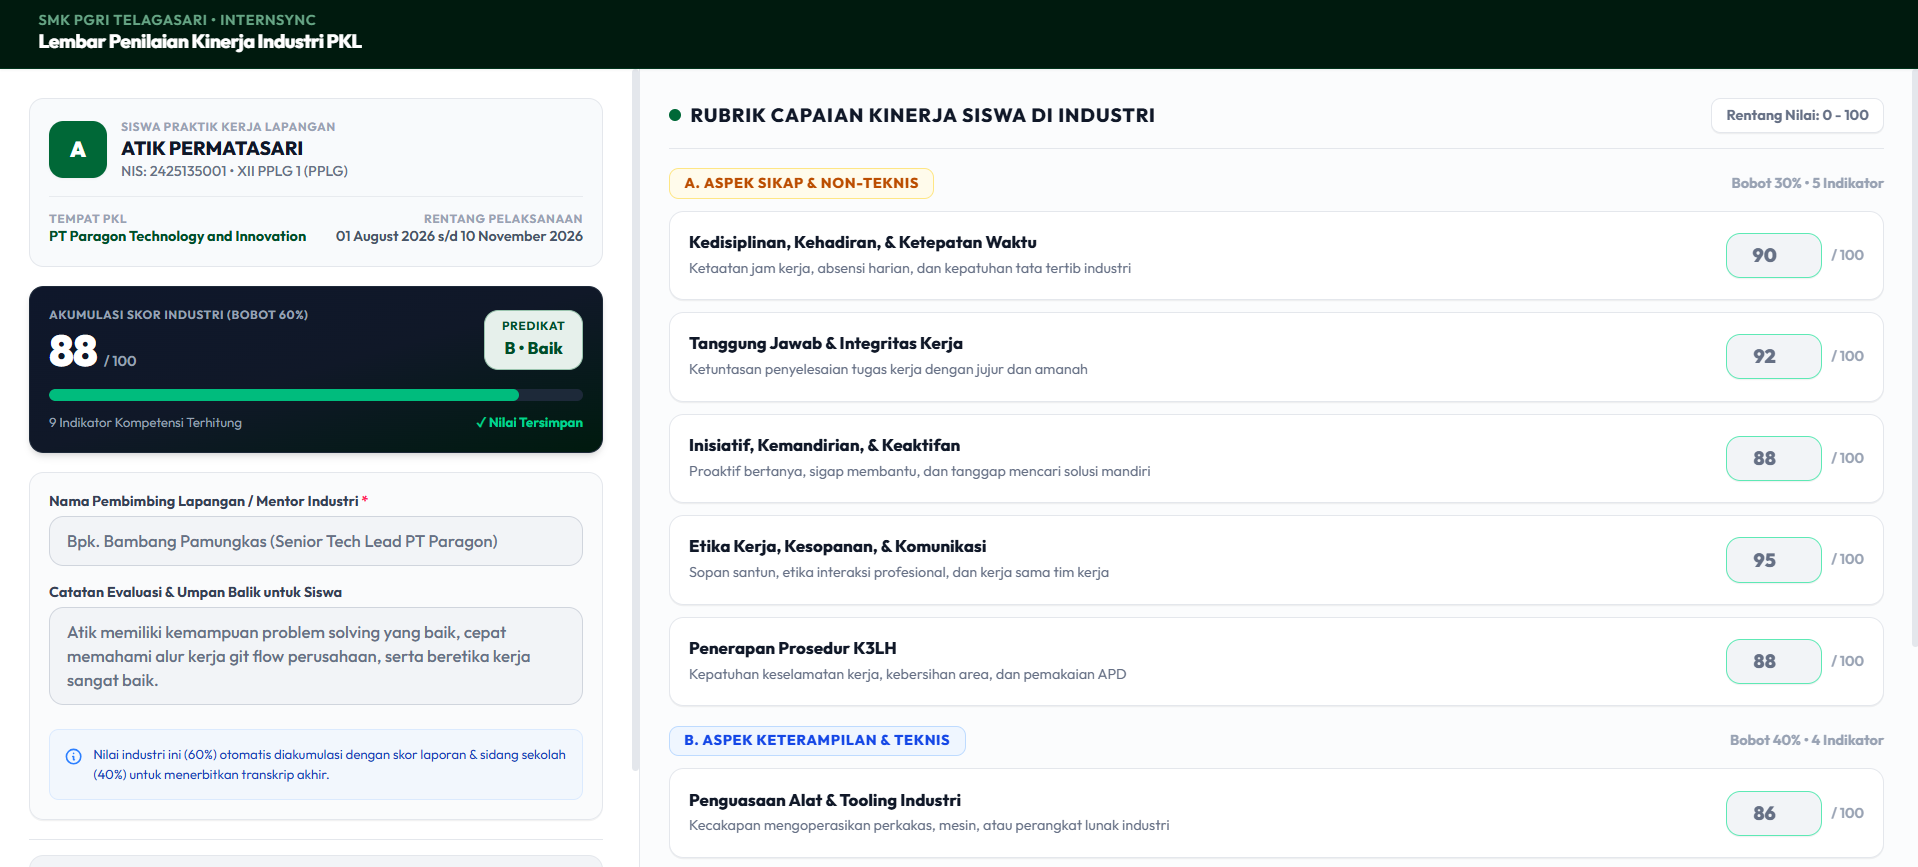
\includegraphics[width=14.00cm,height=0.78\textheight,keepaspectratio]{gambar/gambar-3-28.png}
\caption{Antarmuka Web Publik Penilaian Rubrik Kinerja Industri 60\% (Pembimbing Industri)}\label{fig:3.28}
\end{figure}

Antarmuka ini beroperasi pada rute publik berbasis token \url{/penilaian-industri/:token} yang memungkinkan Pembimbing Industri memberikan penilaian kinerja objektif kepada siswa bimbingannya tanpa autentikasi akun. Formulir menampilkan 9 indikator rubrik baku evaluasi magang SMK dalam dua kelompok: aspek sikap dan non-teknis (kedisiplinan dan kehadiran, tanggung jawab dan integritas kerja, inisiatif dan kemandirian, etika kerja dan komunikasi, serta penerapan K3LH) dan aspek keterampilan dan teknis (penguasaan peralatan dan tooling industri, kualitas dan presisi hasil pekerjaan, analisis dan pemecahan masalah, serta kecepatan dan ketuntasan tugas). Nilai diinputkan pada kolom numerik 0–100, dan sistem menampilkan akumulasi skor industri yang berkontribusi 60\% terhadap nilai akhir PKL siswa. Dua indikator lainnya, yaitu aspek akademik dan laporan, dinilai oleh Guru Pembimbing (Gambar 3.29).

\begin{figure}[H]
\centering
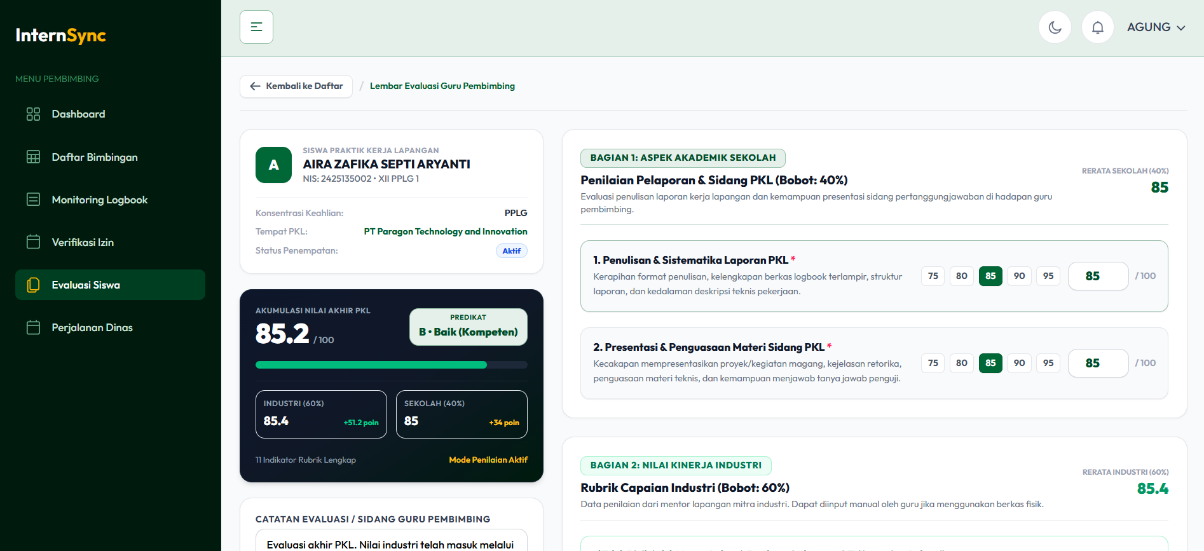
\includegraphics[width=13.89cm,height=0.78\textheight,keepaspectratio]{gambar/gambar-3-29.png}
\caption{Antarmuka Manajemen dan Input Penilaian Sekolah 40\% (Guru Pembimbing)}\label{fig:3.29}
\end{figure}

Halaman Lembar Evaluasi Guru Pembimbing ini digunakan untuk menginput nilai akademik sekolah sekaligus memfinalisasi nilai akhir PKL siswa bimbingan. Sisi kiri menampilkan kartu profil siswa (nama, NIS, kelas, konsentrasi keahlian, dan tempat PKL), kartu Akumulasi Nilai Akhir PKL yang menghitung skor gabungan secara \textit{real-time} beserta predikat kelulusan (misalnya \texttt{85.2 / 100 -- Predikat B Baik (Kompeten)}) dan kontribusi poin Industri 60\% versus Sekolah 40\%, serta kolom catatan evaluasi sidang. Sisi kanan menampilkan formulir Bagian 1: Aspek Akademik Sekolah (Bobot 40\%) untuk memberi skor melalui tombol cepat atau input angka 0--100 pada komponen Penulisan dan Sistematika Laporan PKL serta Presentasi dan Penguasaan Materi Sidang PKL, disertai ringkasan Bagian 2: Nilai Kinerja Industri (Bobot 60\%) dari pembimbing lapangan.

\begin{figure}[H]
\centering
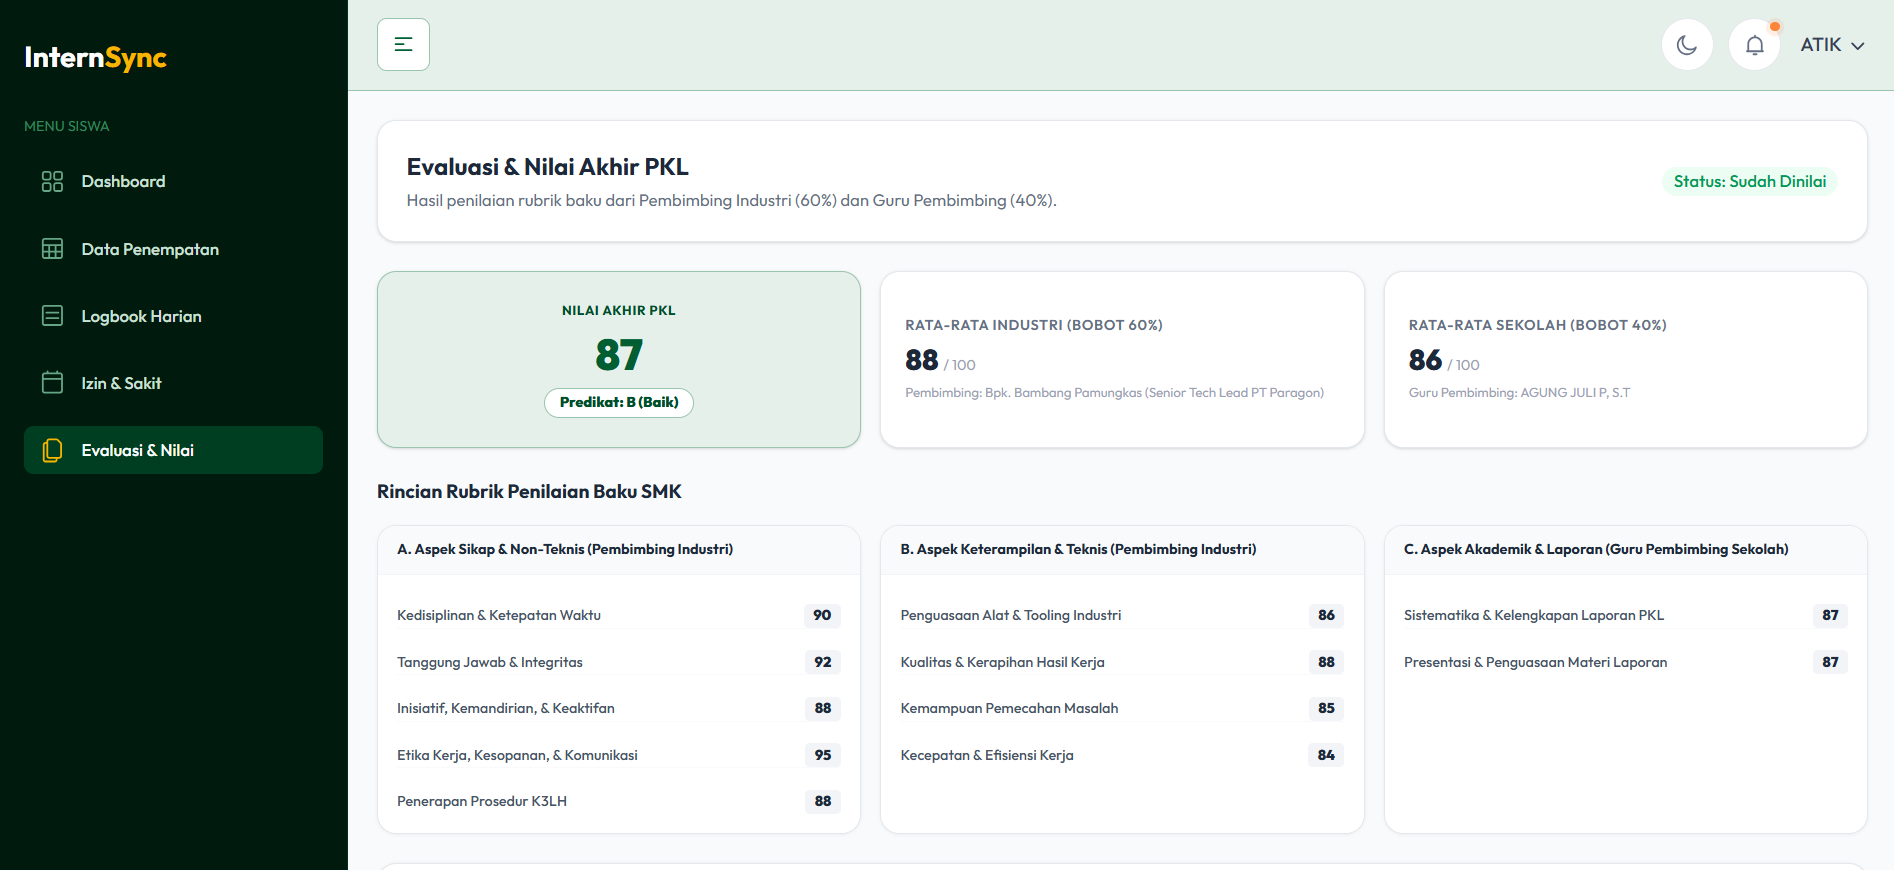
\includegraphics[width=14.00cm,height=0.78\textheight,keepaspectratio]{gambar/gambar-3-30.png}
\caption{Antarmuka Akses Hasil Evaluasi dan Lembar Nilai Akhir Siswa (Published)}\label{fig:3.30}
\end{figure}

Antarmuka pada menu Evaluasi \& Nilai ini menyajikan hasil akhir PKL setelah penilaian difinalisasi oleh Pembimbing Industri dan Guru Pembimbing Sekolah, ditandai dengan \textit{badge} Status: Sudah Dinilai. Bagian atas menampilkan kartu Nilai Akhir PKL beserta predikat, Rata-rata Industri (Bobot 60\%) beserta nama mentor lapangan, dan Rata-rata Sekolah (Bobot 40\%) beserta nama guru pembimbing. Di bagian bawah disajikan rincian skor 11 indikator dalam tiga kelompok: aspek sikap dan non-teknis (Pembimbing Industri), aspek keterampilan dan teknis (Pembimbing Industri), serta aspek akademik dan laporan (Guru Pembimbing Sekolah). Siswa dapat mengunduh lembar nilai resmi berformat PDF ber-QR Code untuk menjamin keaslian dokumen.

\begin{figure}[H]
\centering
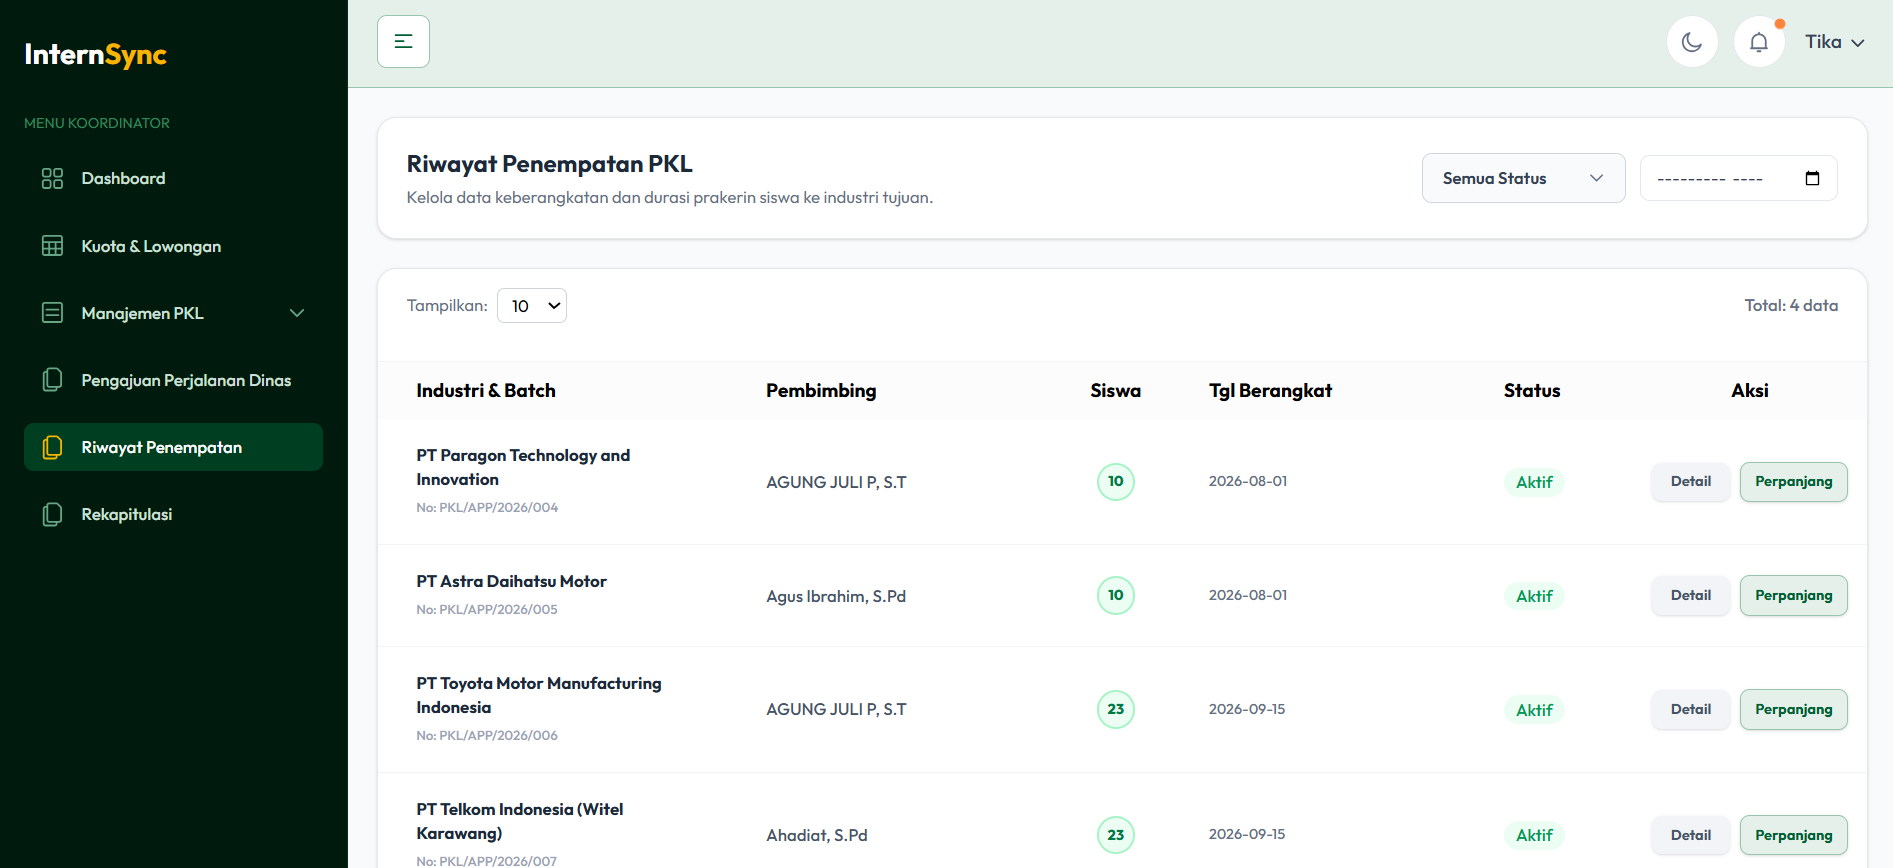
\includegraphics[width=14.00cm,height=0.78\textheight,keepaspectratio]{gambar/gambar-3-31.png}
\caption{Antarmuka Riwayat Penempatan dan Pengelolaan Durasi PKL (Koordinator)}\label{fig:3.31}
\end{figure}

Antarmuka ini berfungsi sebagai pusat pemantauan riwayat keberangkatan dan pengelolaan durasi penempatan PKL oleh Koordinator. Komponen utamanya berupa \textit{data table} yang merangkum pengiriman per kelompok (\textit{batch}) berdasarkan industri tujuan dan nomor dokumen pengajuan, guru pembimbing, jumlah siswa, tanggal keberangkatan, serta status pelaksanaan (Aktif/Selesai). Halaman ini dilengkapi filter status dan periode keberangkatan, serta tombol Detail untuk meninjau siswa dan Perpanjang untuk memperbarui masa PKL.

\section{RENCANA PENGEMBANGAN APLIKASI MOBILE (SISWA DAN GURU PEMBIMBING)}

Sebagai pengembangan lanjutan, aplikasi \textit{mobile} direncanakan untuk memfasilitasi mobilitas operasional harian di lapangan bagi peran Siswa dan Guru Pembimbing. Aplikasi ini direncanakan dibangun menggunakan framework Flutter (Dart), yang memungkinkan kompilasi lintas platform menggunakan satu basis kode yang efisien. Pada proyek akhir ini, fokus implementasi adalah aplikasi web, sedangkan aplikasi \textit{mobile} masih berada pada tahap perencanaan dan belum direalisasikan. Aplikasi \textit{mobile} tidak dirancang sebagai entitas independen, melainkan direncanakan beroperasi sebagai \textit{frontend} seluler yang terintegrasi langsung dengan \textit{backend} Laravel melalui arsitektur RESTful API yang sama dengan aplikasi web. Pendekatan ini lazim diterapkan pada pengembangan aplikasi \textit{mobile} berbasis Flutter yang mengandalkan REST API sebagai jembatan komunikasi data dengan \textit{backend}, sebagaimana diterapkan pada penelitian pengembangan aplikasi \textit{reimbursement} berbasis Android \cite{ref16}. Autentikasi berbasis token yang telah diimplementasikan melalui Laravel Sanctum pada aplikasi web juga sejalan dengan praktik umum penerapan \textit{Bearer Token}/JSON Web Token (JWT) pada arsitektur REST API untuk menjamin keamanan sesi pengguna \cite{ref17}, dan dapat digunakan kembali oleh aplikasi \textit{mobile}.

Pendekatan \textit{client-server} berbasis REST API terpusat ini diharapkan menjaga konsistensi dan integritas data antara platform \textit{web} dan \textit{mobile}. Fungsionalitas aplikasi \textit{mobile} direncanakan difokuskan pada kepraktisan pelaporan harian siswa di lokasi magang serta kemudahan pengawasan Guru Pembimbing di lapangan dengan rencana fitur sebagai berikut:

\begin{enumerate}[label=\alph*.]
\item \textbf{Autentikasi Terpusat dan Keamanan Sesi}
\par\noindent Sistem login direncanakan menggunakan kredensial (Email/NIP/NIS dan kata sandi) yang sama dengan versi \textit{web}. Autentikasi direncanakan memanfaatkan \textit{Bearer Token} berbasis REST (Laravel Sanctum) untuk mengelola sesi secara aman dan mengarahkan tampilan aplikasi sesuai peran pengguna (Siswa atau Guru Pembimbing) tanpa perlu login berulang kali.
\item \textbf{Dasbor Ringkas (\textit{Executive Summary})}
\par\noindent Dasbor direncanakan menyajikan metrik esensial sesuai peran pengguna. Bagi siswa, dasbor menampilkan persentase progres durasi PKL dan total catatan \textit{logbook} harian yang telah diisi. Bagi Guru Pembimbing, dasbor menampilkan total siswa bimbingan aktif, permohonan izin \textit{fallback} yang perlu ditinjau, serta jadwal kunjungan terdekat.
\item \textbf{Pencatatan dan Pemantauan Logbook Harian}
\par\noindent Siswa direncanakan dapat mencatat aktivitas kerja harian secara mandiri (\textit{self-reporting}) dan mengunggah foto dokumentasi kegiatan langsung dari kamera ponsel saat berada di lokasi industri. Guru Pembimbing direncanakan dapat memantau riwayat aktivitas harian dan memeriksa lampiran bukti kegiatan siswa bimbingannya melalui ponsel.
\item \textbf{Pengajuan Izin/Sakit dan Mekanisme Fallback Presensi}
\par\noindent Siswa direncanakan dapat mengajukan permohonan izin atau sakit beserta unggahan foto surat keterangan dokter dan membagikan tautan token konfirmasi kepada Pembimbing Industri melalui WhatsApp. Guru Pembimbing direncanakan dapat memverifikasi izin melalui mekanisme \textit{fallback} apabila pihak industri belum merespons dalam waktu 24 jam.
\item \textbf{Pemantauan Progres dan Evaluasi Lapangan}
\par\noindent Aplikasi direncanakan menampilkan daftar siswa di bawah supervisi Guru Pembimbing beserta lokasi industri dan indikator penyelesaian durasi PKL, serta memfasilitasi input nilai pembimbingan sekolah (40\%) dan peninjauan hasil evaluasi akhir saat supervisi kunjungan industri.
\end{enumerate}

Desain antarmuka (UI/UX) aplikasi \textit{mobile} direncanakan berfokus pada kemudahan navigasi dan efisiensi interaksi (\textit{user-friendly}), dengan menghindari elemen visual berlebihan agar aplikasi tetap ringan dijalankan pada berbagai spesifikasi perangkat ponsel siswa maupun tenaga pendidik. Hingga aplikasi \textit{mobile} terealisasi, kebutuhan mobilitas tersebut dilayani oleh antarmuka web responsif yang telah diuji pada resolusi ponsel (subbab 4.7).

\section{RENCANA PENGUJIAN SISTEM}

Untuk menjamin keandalan, stabilitas, dan kesesuaian sistem InternSync dengan kebutuhan pengguna di SMK PGRI Telagasari, pengujian perangkat lunak akan dilakukan menggunakan metode Black Box Testing. Fokus pengujian murni berada pada validasi fungsionalitas input dan output dari perspektif pengguna akhir, tanpa perlu menganalisis atau membongkar struktur kode internal (source code) \cite{ref18}.

Metode Black Box Testing dipilih karena memungkinkan pengujian dilakukan murni dari sudut pandang pengguna akhir tanpa memerlukan pengetahuan teknis terhadap struktur kode program \cite{ref19}. Salah satu teknik yang umum digunakan dalam pendekatan ini adalah analisis nilai batas (boundary value analysis), yang efektif untuk menguji validitas input pada kondisi-kondisi ekstrem seperti batas ukuran file atau format data numerik \cite{ref20}.

Skenario pengujian komprehensif ini dirancang untuk mencakup beberapa parameter operasional utama:

\begin{enumerate}[label=\alph*.]
\item Pengujian Autentikasi dan Manajemen Hak Akses (Role-Based Access Control):
\begin{itemize}
\item Memastikan secara ketat bahwa setiap aktor (Siswa, Guru Pembimbing, Koordinator, Hubin, Admin) hanya diizinkan mengakses menu, data, dan fungsi yang sesuai dengan kewenangan spesifiknya.
\item Menguji limitasi keamanan rute aplikasi. Misalnya, mencoba memaksa masuk menggunakan akun siswa ke URL yang dikhususkan untuk dasbor Hubin, di mana sistem harus secara otomatis memblokir akses dan mengarahkan pengguna kembali ke halaman yang diizinkan.
\end{itemize}
\item Pengujian Fungsionalitas Inti (CRUD Operations):
\begin{itemize}
\item Modul Katalog Lowongan dan Pengajuan PKL: Memvalidasi alur pembuatan lowongan oleh Koordinator, pemilihan lowongan oleh Siswa, seleksi pendaftar, hingga pengajuan dan persetujuan akhir oleh Hubin berjalan tanpa galat.
\item Modul Logbook Harian dan Perizinan: Menguji form input catatan aktivitas mandiri oleh siswa, proses unggah bukti, penguncian tanggal otomatis saat izin/sakit disetujui, serta ekspor rekapitulasi PDF ber-QR Code oleh Guru Pembimbing.
\item Modul Evaluasi Akhir: Memastikan nilai rubrik industri (60\%) dan nilai sekolah (40\%) diproses secara matematis dengan benar, termasuk validasi input anomali (seperti karakter non-numerik atau angka negatif).
\end{itemize}
\item Pengujian Responsivitas Antarmuka:
\begin{itemize}
\item Memastikan tampilan aplikasi web menyesuaikan dengan baik pada berbagai ukuran layar (desktop, laptop, tablet, dan ponsel) tanpa distorsi tata letak maupun gulir horizontal, karena kebutuhan akses dari perangkat ponsel pada tahap ini dilayani oleh antarmuka web responsif.
\end{itemize}
\item Pengujian Penanganan Kesalahan (Error Handling):
\begin{itemize}
\item Menguji respon sistem saat dihadapkan pada interaksi pengguna yang tidak standar, seperti tidak mengisi kolom wajib pada form pengajuan, atau mengunggah file yang melampaui batas ukuran maksimal server. Sistem diwajibkan menampilkan pesan peringatan (error message) yang jelas dan informatif.
\end{itemize}
\end{enumerate}
